\documentclass[10pt,a4paper,titlepage,oneside,final]{book}
\usepackage[english]{babel}
\usepackage[utf8x]{inputenc}
\usepackage[T1]{fontenc}
\usepackage{lmodern}
\usepackage[a4paper,textwidth=345pt,textheight=598pt,hmarginratio=1:1]{geometry}
\usepackage[final]{graphicx}
\usepackage{subfigure}
\usepackage[intlimits]{amsmath}
\usepackage{amssymb}
\usepackage{booktabs}
\usepackage{microtype}
\usepackage{float}
\usepackage[pdfborder={0 0 0}]{hyperref}
\usepackage{cleveref}
%\usepackage{siunitx}
\usepackage{tabularx}
\usepackage{caption}
\usepackage{ragged2e}
\usepackage{soul}
\usepackage{theorem}
%\usepackage{pgfplots}
%\usepackage{nameref}
\usepackage{tikz}
%\usetikzlibrary{shapes,calc,automata}
%\usepackage{rotating}
%\usepackage{listings}
%\usepackage{nicefrac}
\usepackage{makeidx}
\usepackage{paralist}

\usepackage{placeins}

\makeatletter

\captionsetup{format=hang,justification=justified,labelfont=bf,labelsep=colon,font=small}
\long\def\clap#1{\hbox to 0pt{\hss#1\hss}}

\author{Patrik Fimml\and NeroBurner}
\title{Lecture Notes 2013W\\ 104.271 Discrete Mathematics VO\\ (Gittenberger)}

\makeindex
\gdef\th@custom{%
  \th@plain%
  \def\@begintheorem##1##2{%
    \item[\hskip\labelsep \theorem@headerfont ##1\ ##2.]}}%
\theoremstyle{custom}
\theorembodyfont{\normalfont}
\newtheorem{definition}{Definition}

\def\thechapter{\Roman{chapter}}

\parindent=0pt
\parskip=\medskipamount

\pltopsep=-5pt
\plpartopsep=0pt

\def\TODO#1{\fbox{TODO: #1}}


\newcommand{\tikzmark}[2]{\tikz[overlay,remember picture,baseline] \node [anchor=base] (#1) {$#2$};}

\newcommand{\DrawLineHorizontal}[3][]{%
	\begin{tikzpicture}[overlay,remember picture]
		\draw[#1] (#2.west) -- (#3.east);
	\end{tikzpicture}
}
\newcommand{\DrawLine}[3][]{%
	\begin{tikzpicture}[overlay,remember picture]
		\draw[#1] (#2.north) -- (#3.south);
	\end{tikzpicture}
}

\begin{document}
% "defined term"
\def\dt#1{\textbf{#1}}

\def\Remark.{\noindent \textbf{Remark.}}
\def\Lemma.{\noindent \textbf{Lemma.}}
\def\Theorem.{\noindent \textbf{Theorem.}}
\def\Proof.{\noindent \textbf{Proof.}}
\def\ProofForward.{\noindent \textbf{Proof (``$\Rightarrow$'').}}
\def\ProofBackward.{\noindent \textbf{Proof (``$\Leftarrow$'').}}

\maketitle
\tableofcontents
%\listoffigures

% include the chapters here:

\chapter{Graph Theory}
%%%  03.10.2013  %%%
%%%  VO 01
\section{Basics}
\lecturedate[\baselineskip]{2013-10-03}

\begin{definition}
\index{graph}
\index{vertex set}
\index{edge set}
A structure \dt{$G=(V,E)$} is called a \dt{graph}.
$V=\{v_1, v_2, \ldots, v_n\}$ is the \emph{vertex set} of $G$. $E$ is the
\emph{edge set} of $G$.
\end{definition}

\begin{definition}
\index{graph!directed}
\index{edge}
A \dt{directed graph} $G$ has directed edges $e\in E$ of the form
$e=(v,w)$. $e$ is a pair, in particular $(v,w)\ne (w,v)$. $v,w\in V$.
\end{definition}

\begin{definition}
\index{graph!undirected}
\index{edge}
An \dt{undirected graph} $G$ has undirected edges $e\in E$ of the form
$e=\{v,w\}$. $e$ is a set, in particular $e=\{v,w\}=\{w,v\}=vw$. $vw$ is a
shorthand notation.
\end{definition}

\index{loop}
A \dt{loop} is an edge from a vertex to itself.

Graphs can have \textbf{multiple edges}, in which case $E$ is a multiset.

\begin{figure}[htb]
\centering
\begin{tabular}{c c}
\subfigure[directed graph] {
	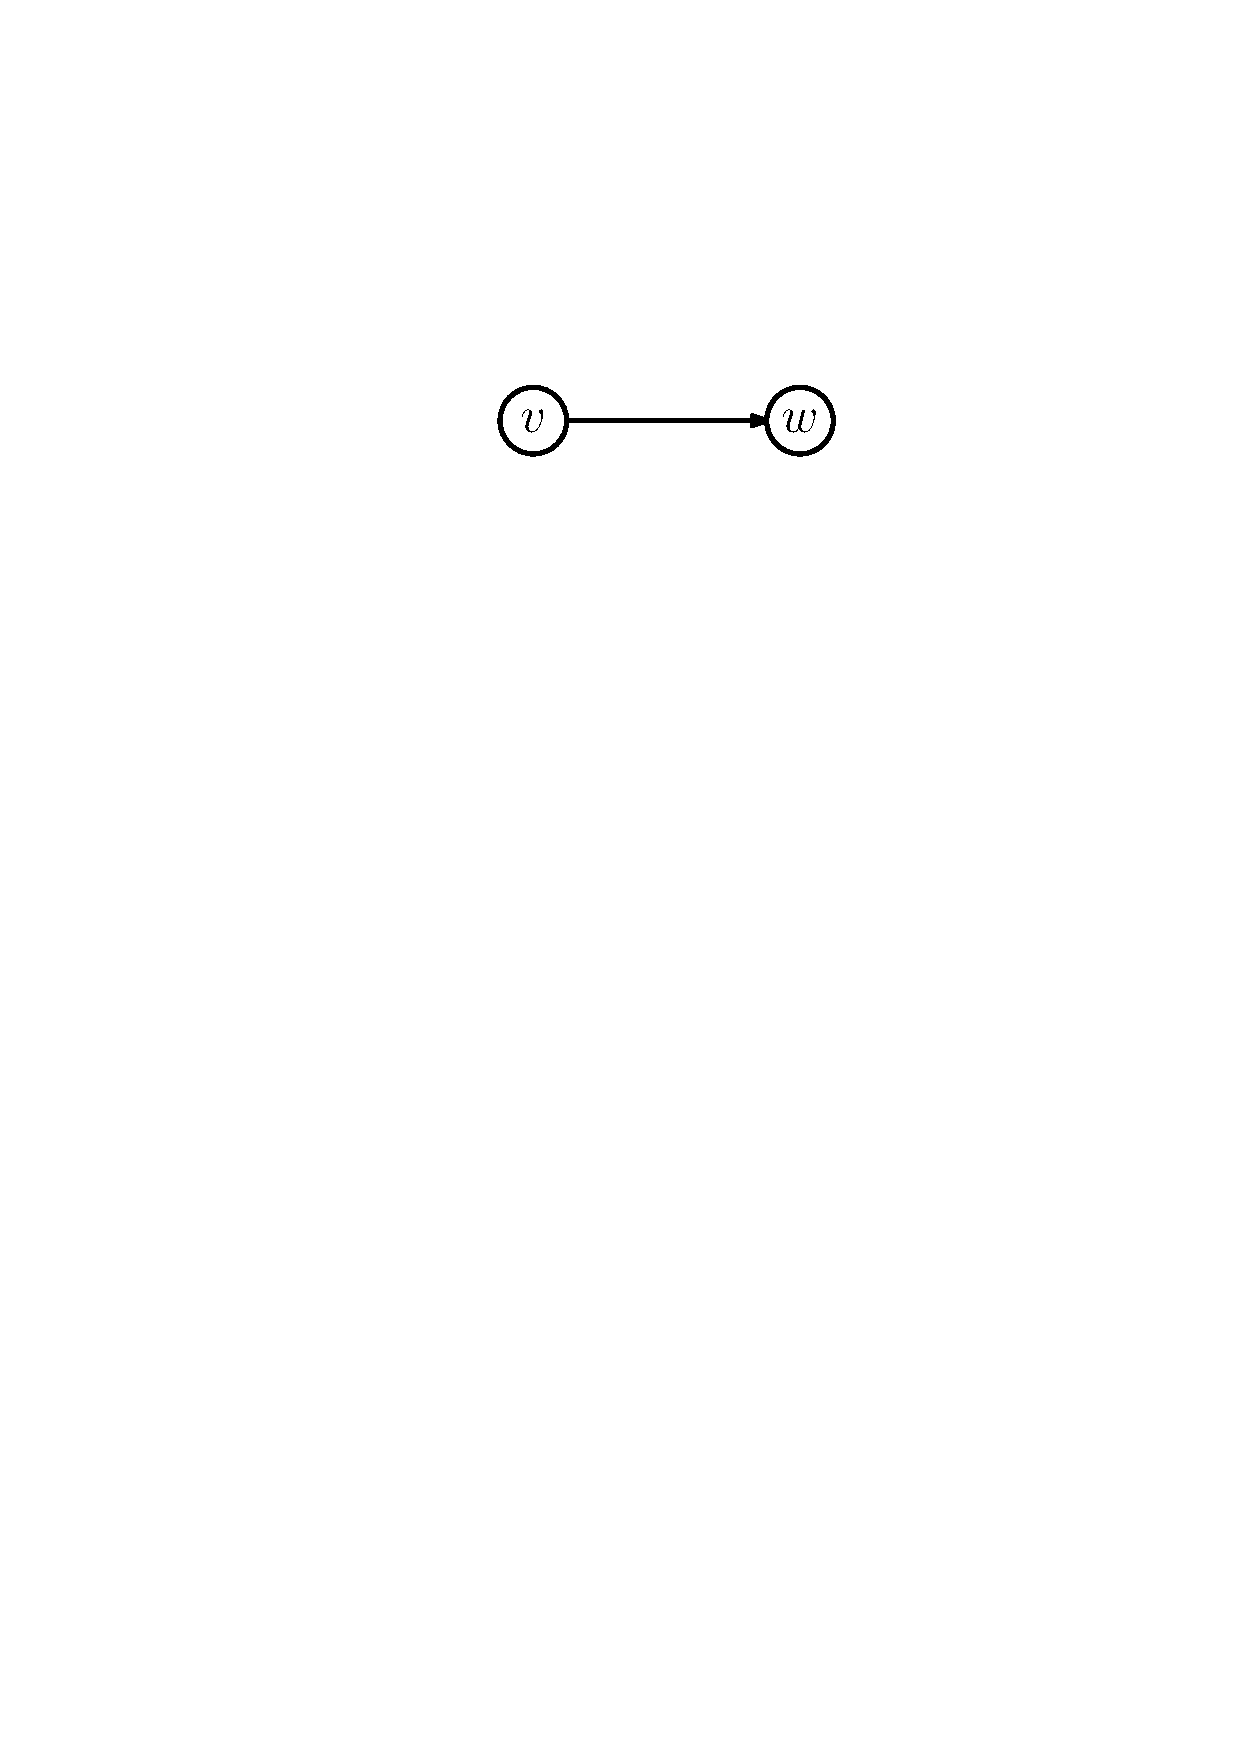
\includegraphics[scale=.5]{01_graph_theory/pics/directed-graph_edge.pdf}
} &
\subfigure[undirected graph] {
	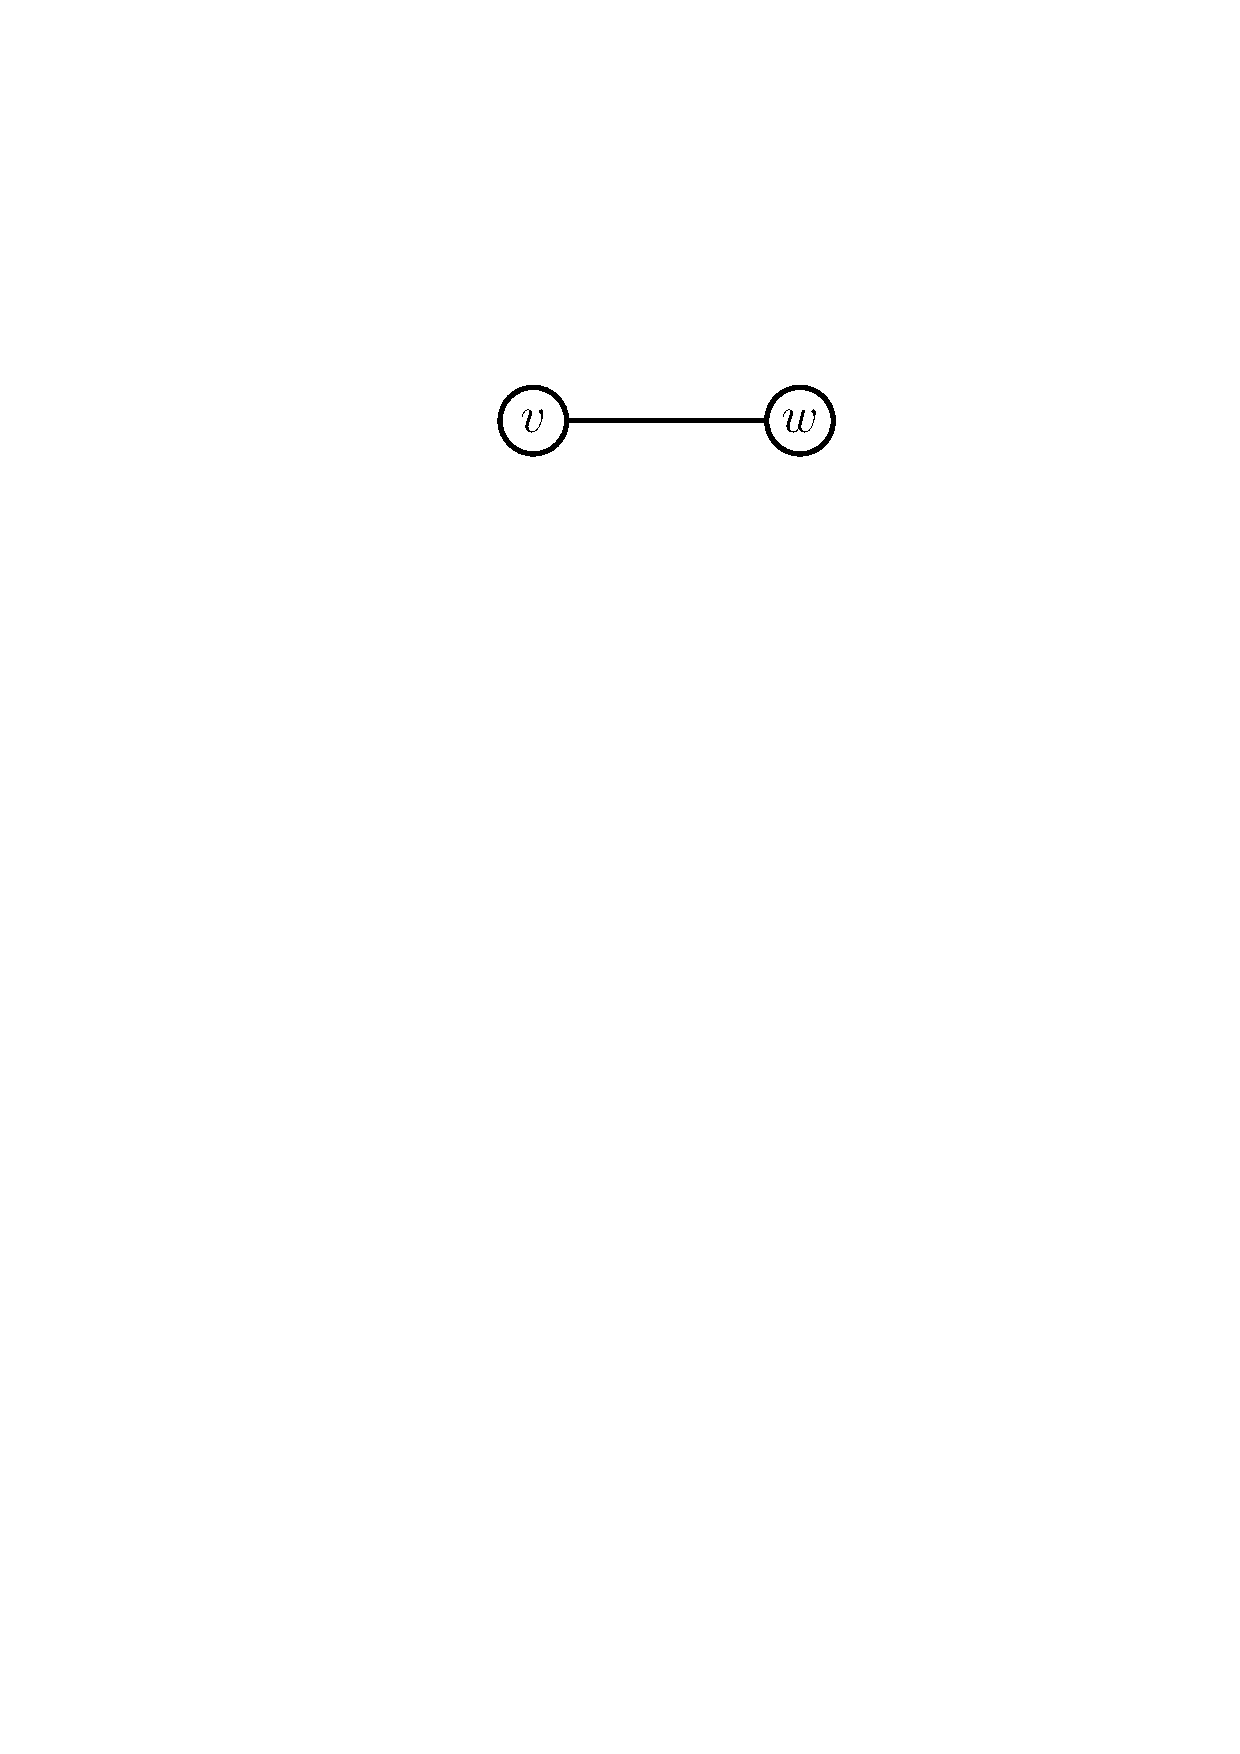
\includegraphics[scale=.5]{01_graph_theory/pics/graph_edge.pdf}
} \\
\subfigure[loop] {
	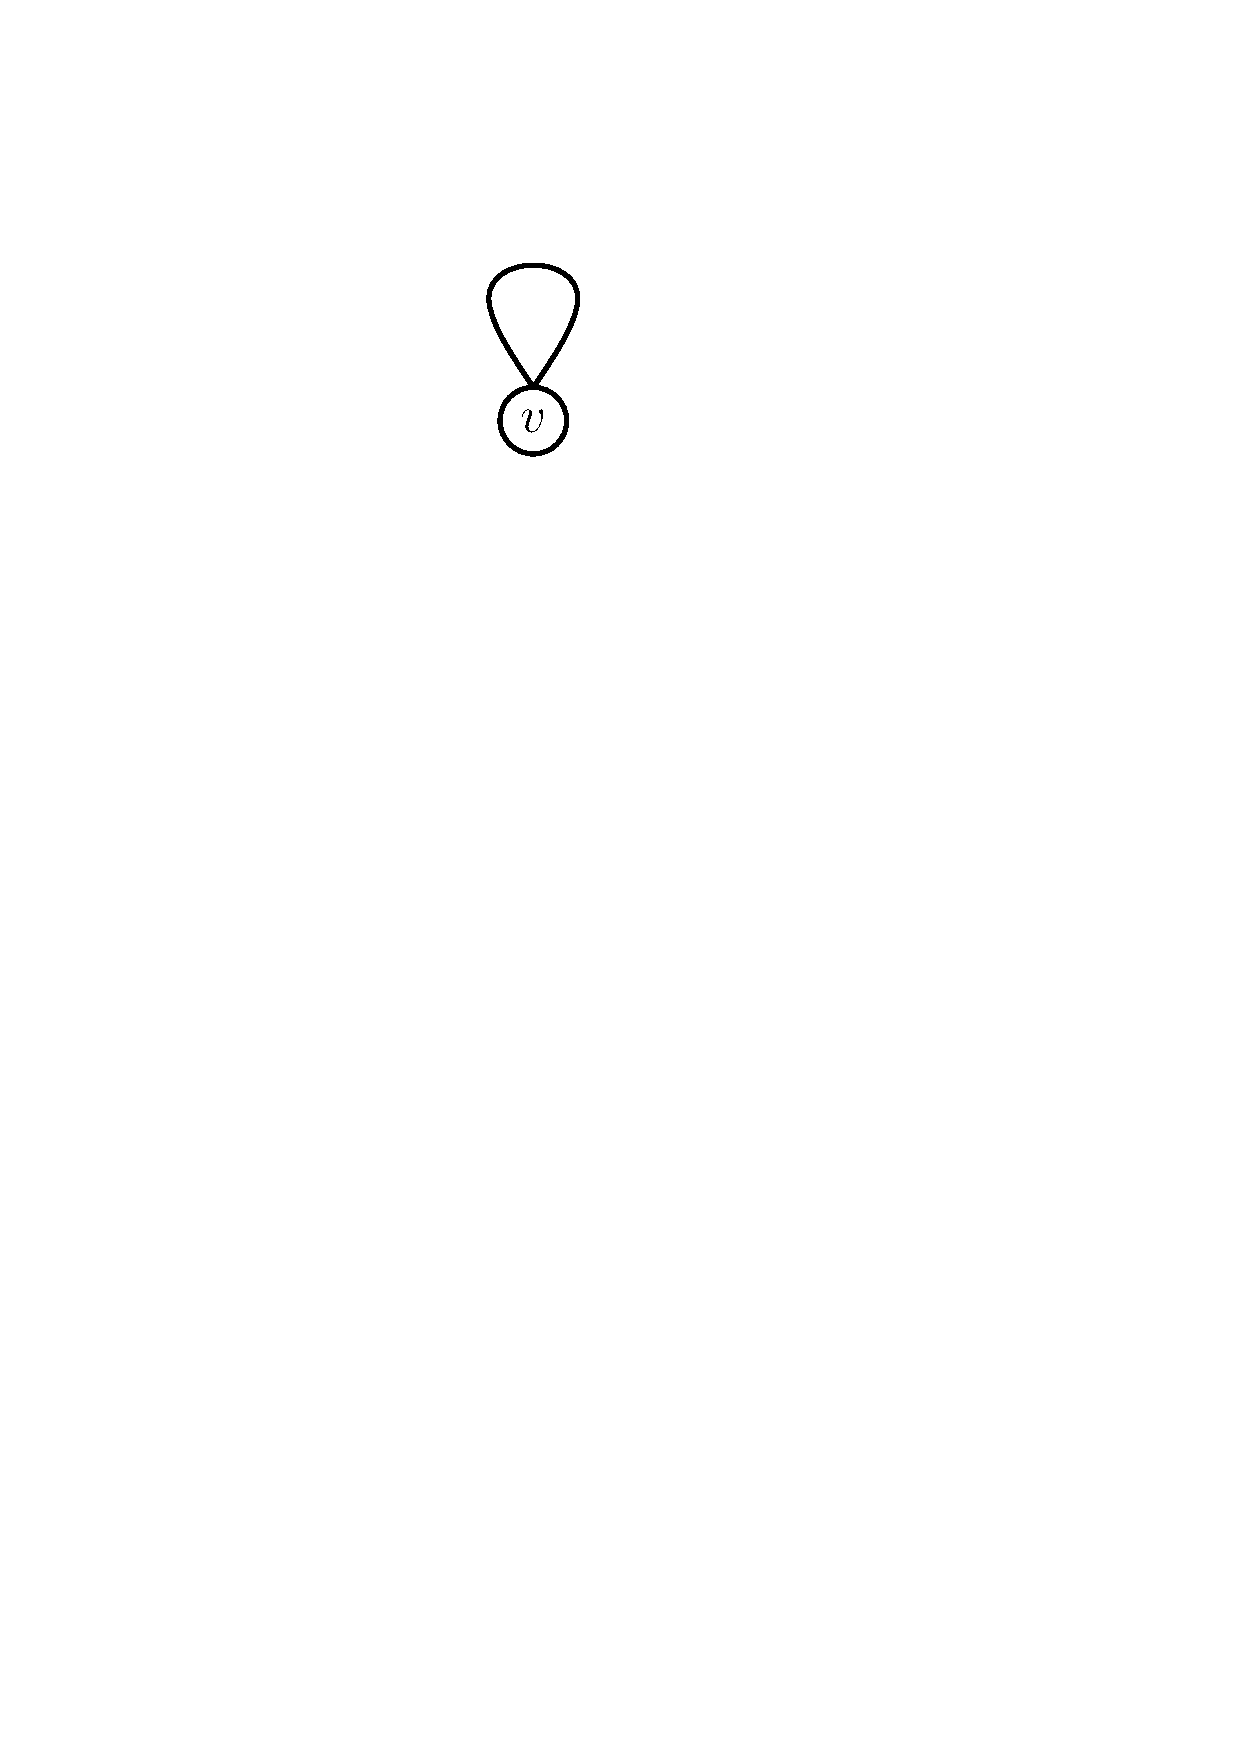
\includegraphics[scale=.5]{01_graph_theory/pics/graph_loop.pdf}
} &
\subfigure[multiple edges] {
	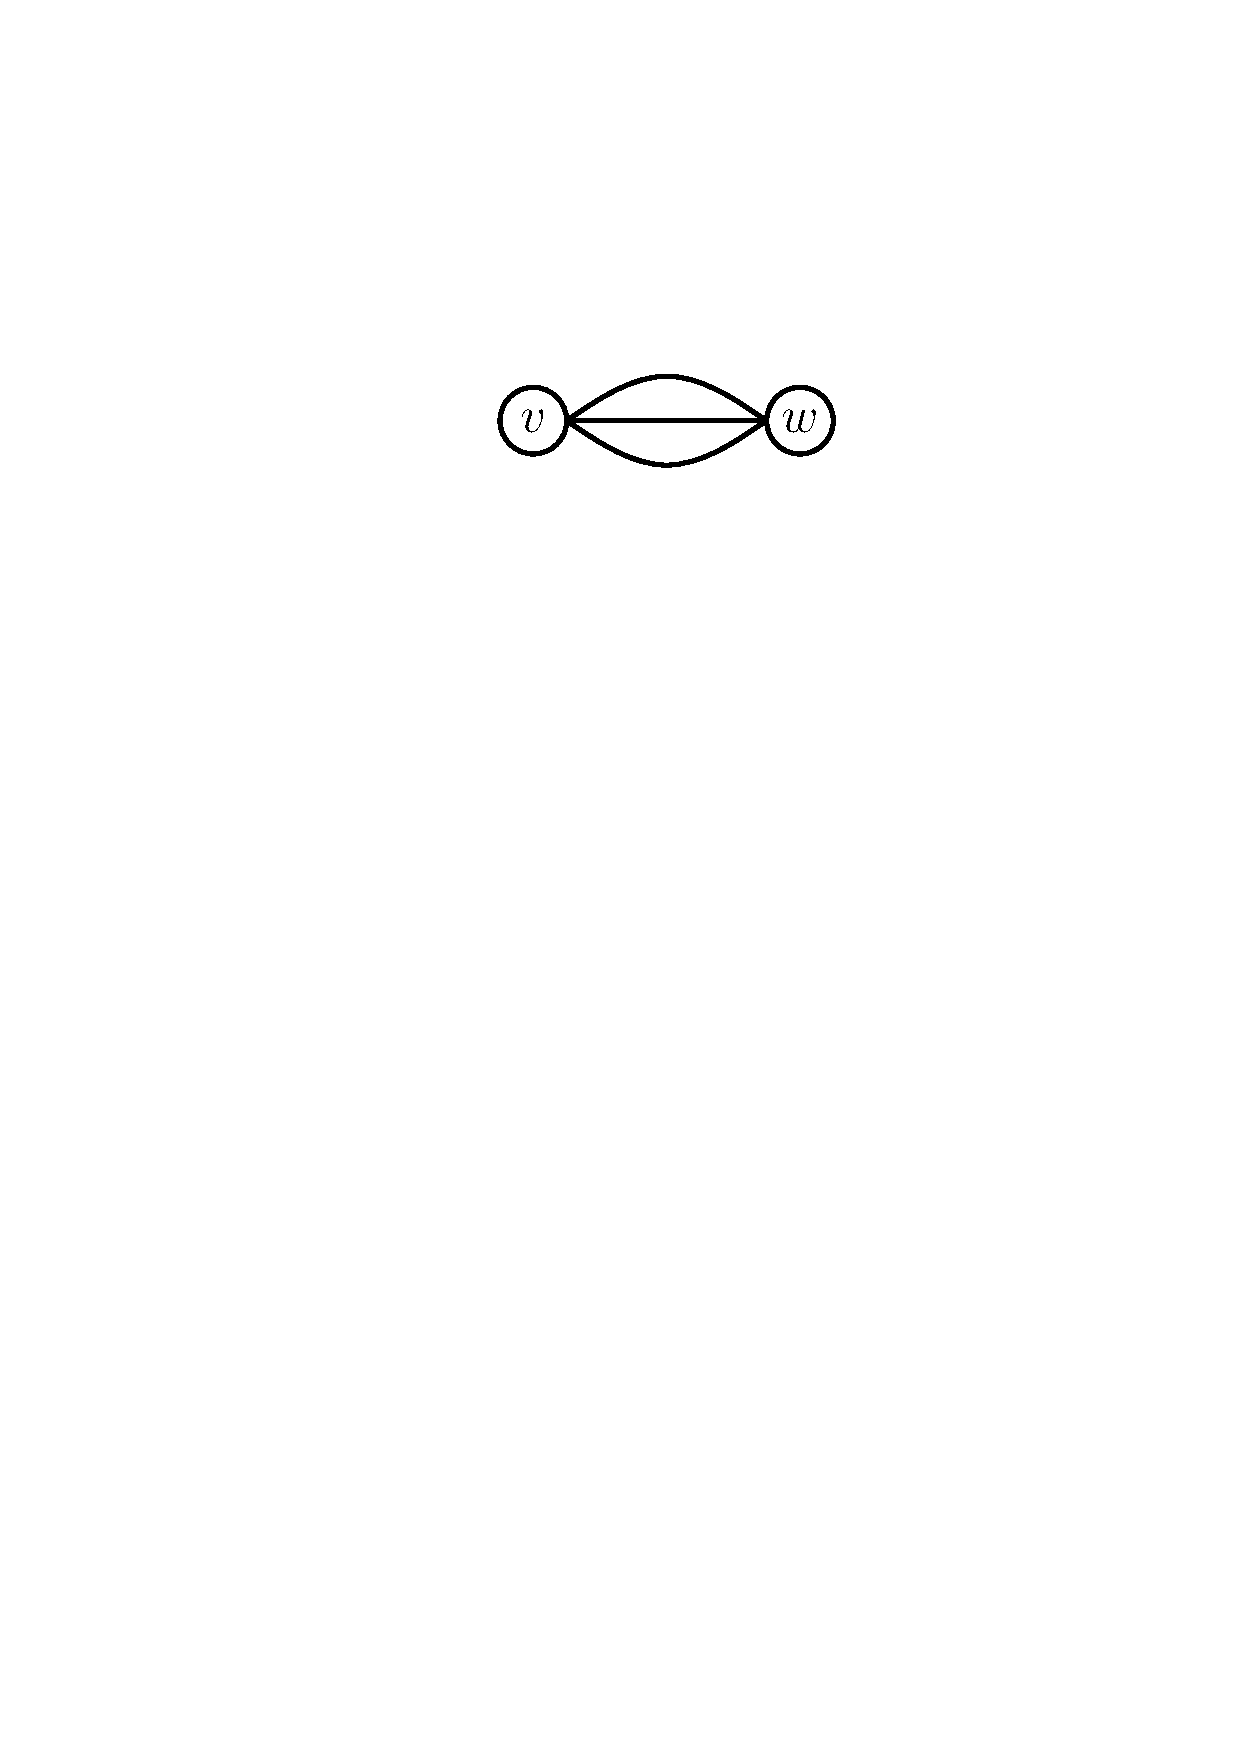
\includegraphics[scale=.5]{01_graph_theory/pics/graph_multiple-edges.pdf}
}
\end{tabular}
\caption{different graphs}
\end{figure}
\FloatBarrier

\begin{definition}
\index{graph!simple}
A graph is \dt{simple} when it has
\begin{compactitem}
\item no loops and 
\item no multiple edges.
\end{compactitem}
\end{definition}

Unless otherwise stated, we assume simple, finite graphs throughout this
lecture.

A graph corresponds to a \emph{relation} on $V$. In case of undirected graphs,
this relation is symmetric.


Notation: \\[\medskipamount]
\begin{tabular}{ll}
  $V$, $V(G)$ & vertice set \\
  $E$, $E(G)$ & edge set \\
  $\alpha_0 = |V|$ & number of vertices \\
  $\alpha_1 = |E|$ & number of edges \\
\end{tabular}

\begin{definition}
\index{degree}
Let $v\in V$. For undirected graphs, 
\begin{compactitem}
  \item the \dt{degree} $d(v)$ is the number of edges \emph{incident} to $v$.
\end{compactitem}
For directed graphs,
\begin{compactitem}
  \item the \dt{out-degree} $d^{+}(v)$ is the number of outgoing edges, i.e. edges of the form $(v,w)$, and
  \item the \dt{in-degree} $d^{-}(v)$ is the number of incoming edges, i.e. edges of the form $(w,v)$.
\end{compactitem}
\end{definition}

\begin{figure}[htb]
\centering
\subfigure[vertex $v$ with degree $d(v)=6$]{
	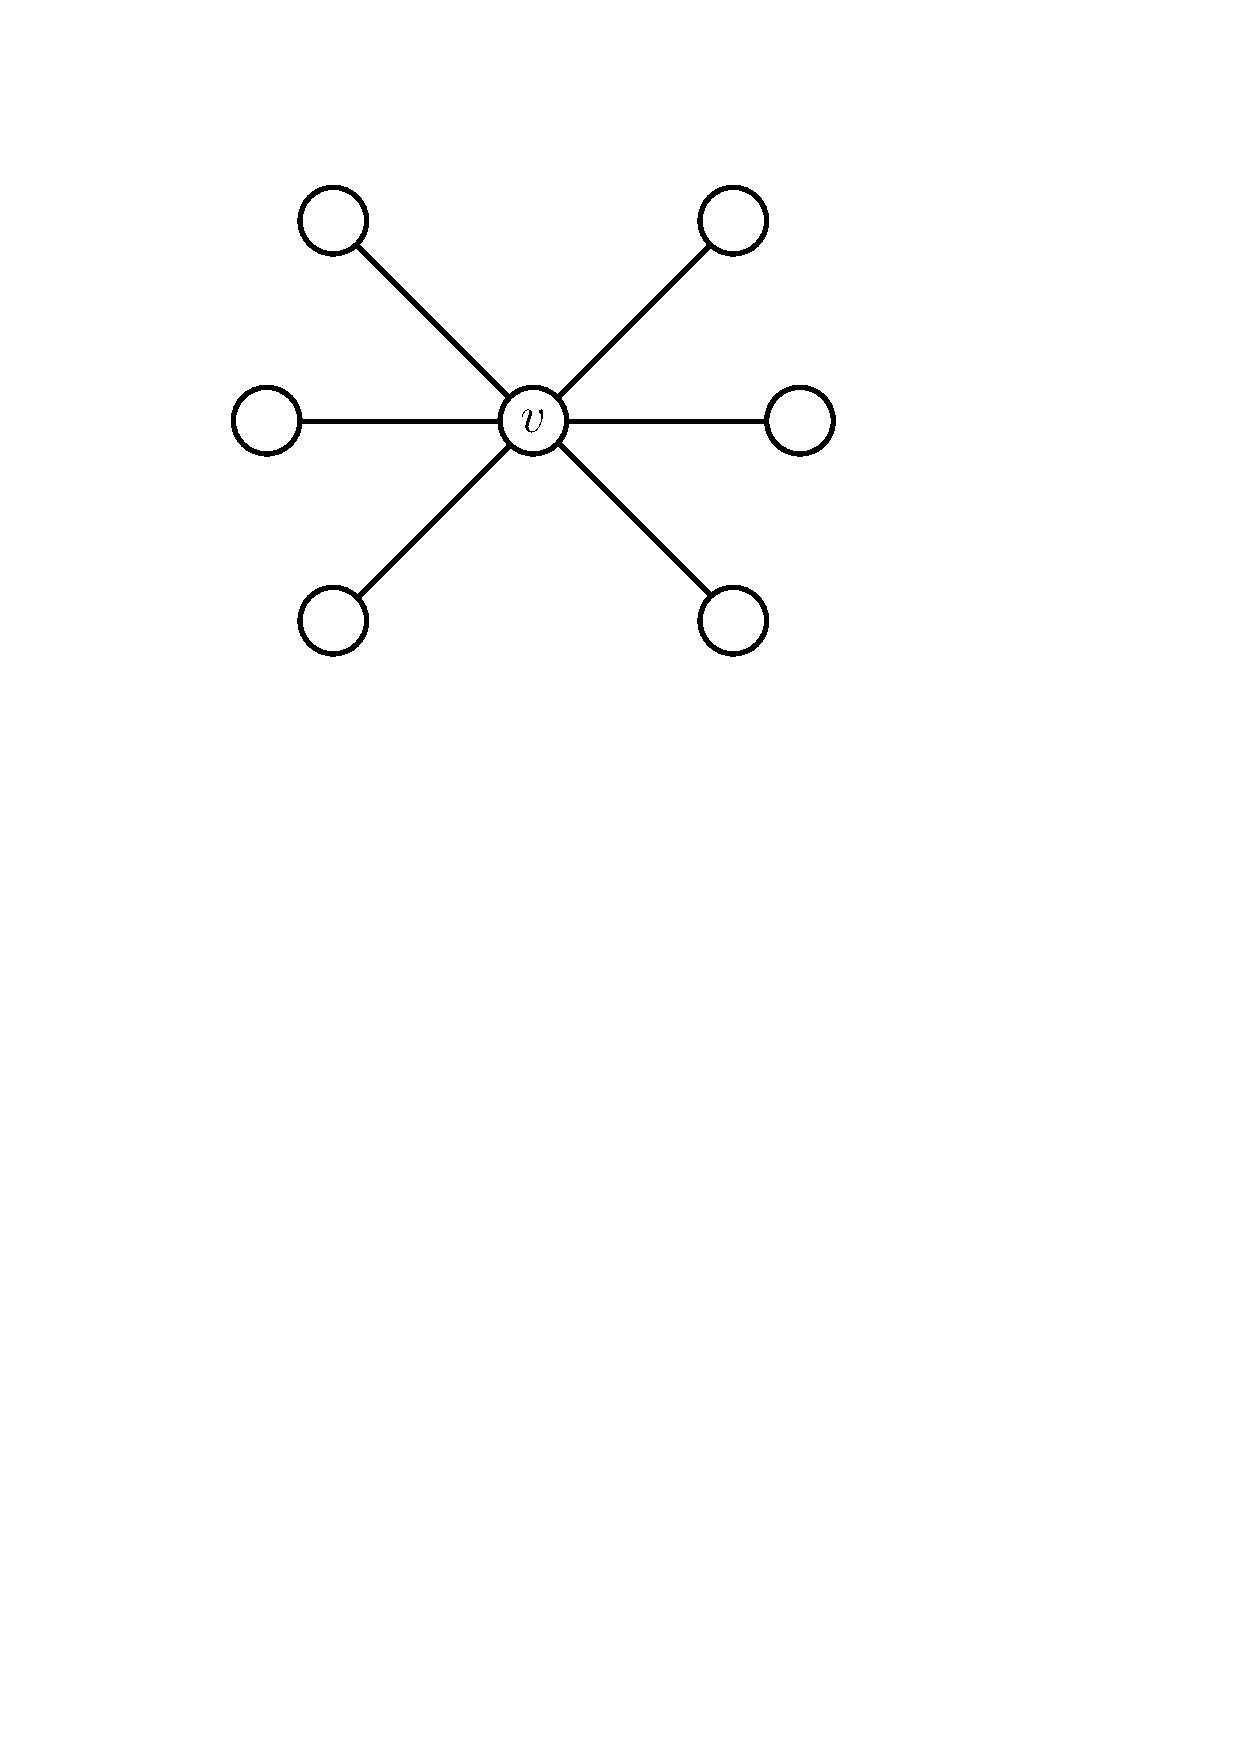
\includegraphics[scale=.5]{01_graph_theory/pics/graph_degree.pdf}
}
\subfigure[vertex $v$ with in-degree $d^{-}(v)=3$ and out-degree $d^{+}(v)=3$]{
	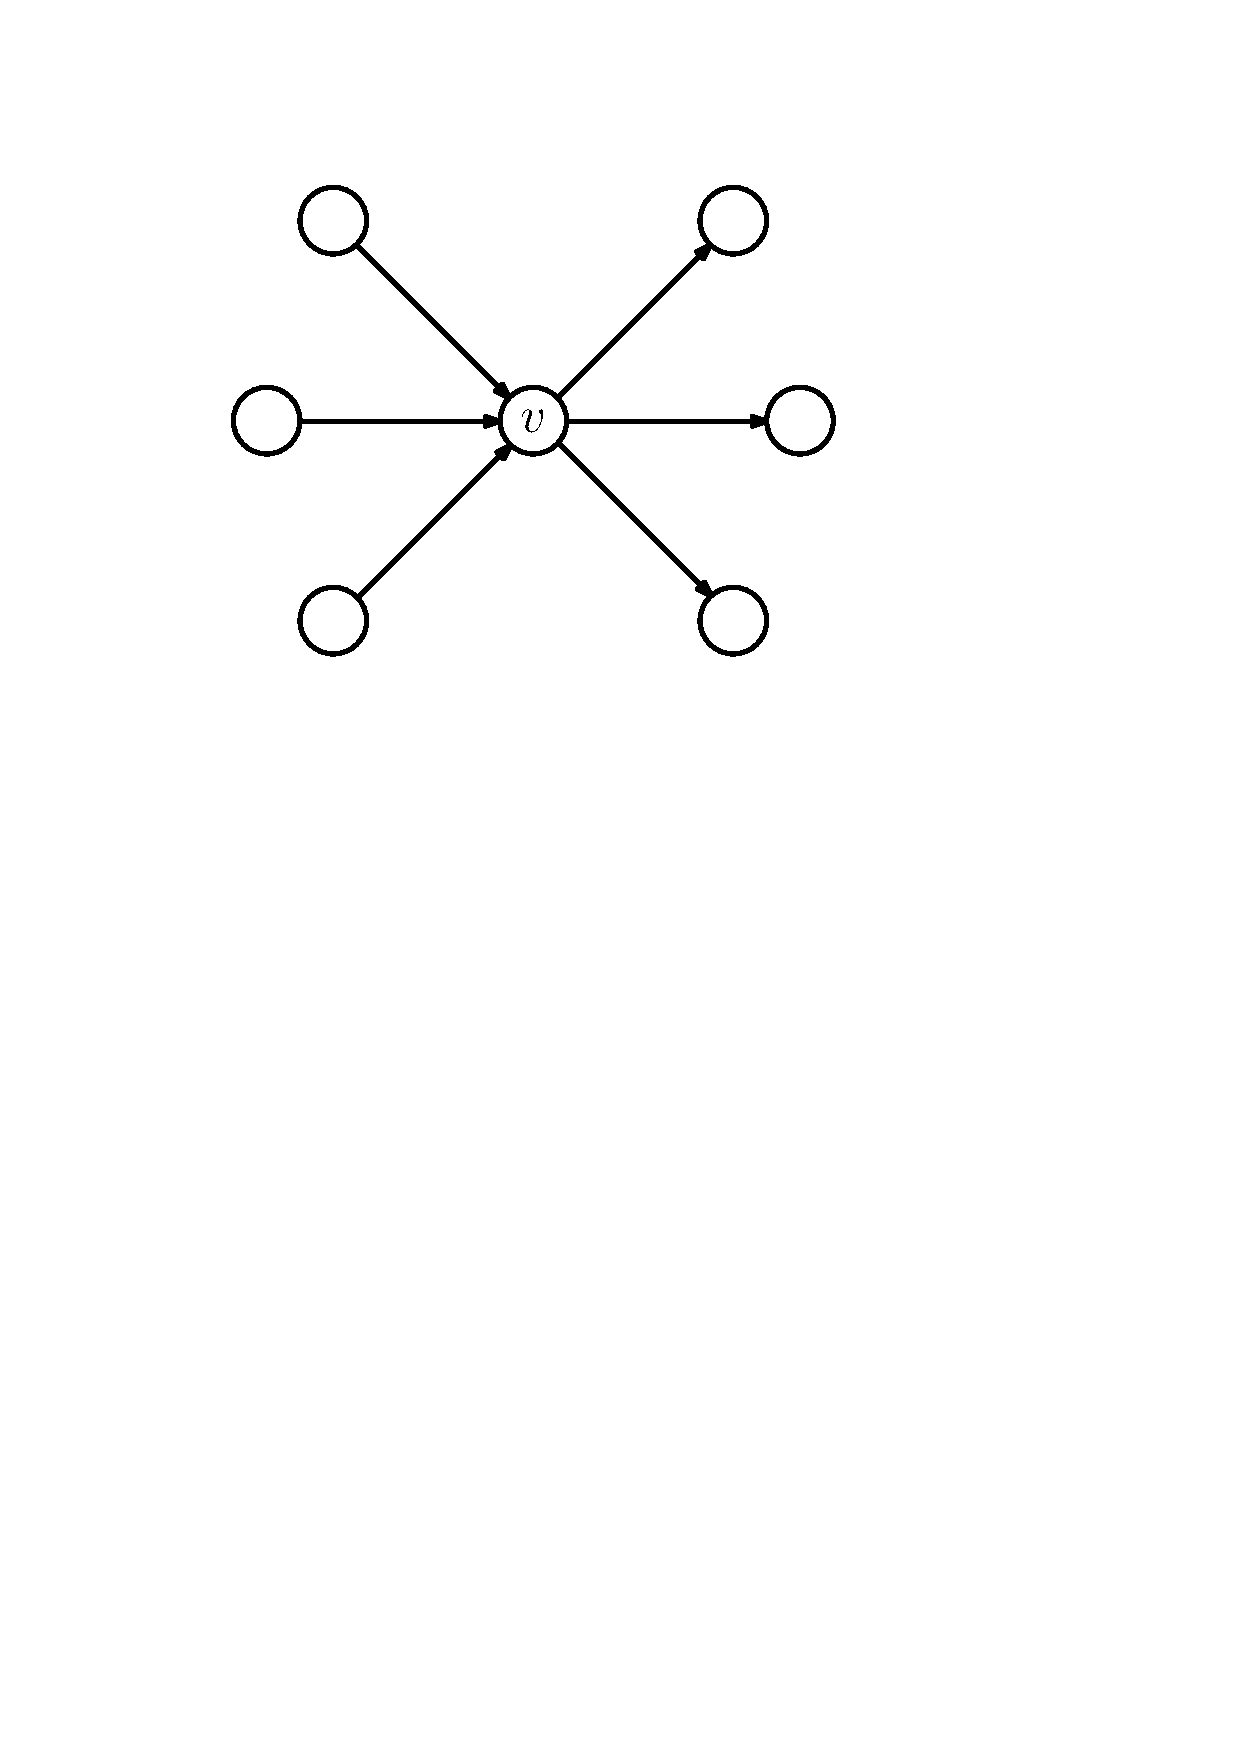
\includegraphics[scale=.5]{01_graph_theory/pics/directed-graph_indegree-outdegree.pdf}
}
\caption{vertex-degrees}
\end{figure}
\FloatBarrier

\begin{definition}
\index{neighbour}
\index{successor}
\index{predecessor}
For undirected graphs,
\begin{compactitem}
\item $\Gamma(v)$ is the \dt{set of neighbours} of $v$.
\end{compactitem}
For directed graphs,
\begin{compactitem}
\item $\Gamma^{+}(v)$ is the \dt{set of successors} of $v$.
\item $\Gamma^{-}(v)$ is the \dt{set of predecessors} of $v$.
\end{compactitem}
\end{definition}

\index{handshaking lemma}
\textbf{Lemma (Handshaking Lemma).} Let $G=(V,E)$ be a simple graph. Then
\begin{align*}
&\sum_{v\in V} d(v) = 2 |E| &&\text{($G$ undirected)} \\
&\sum_{v\in V} d^{+}(v) = \sum{v\in V} d^{-}(v) = |E| &&\text{($G$ directed).} \\
\end{align*}

\textbf{Proof.} see Figure~\ref{fig:hand_shaking_lemma}

\begin{figure}[htb]
\centering
\subfigure[undirected graph, each edge is counted twice]{
	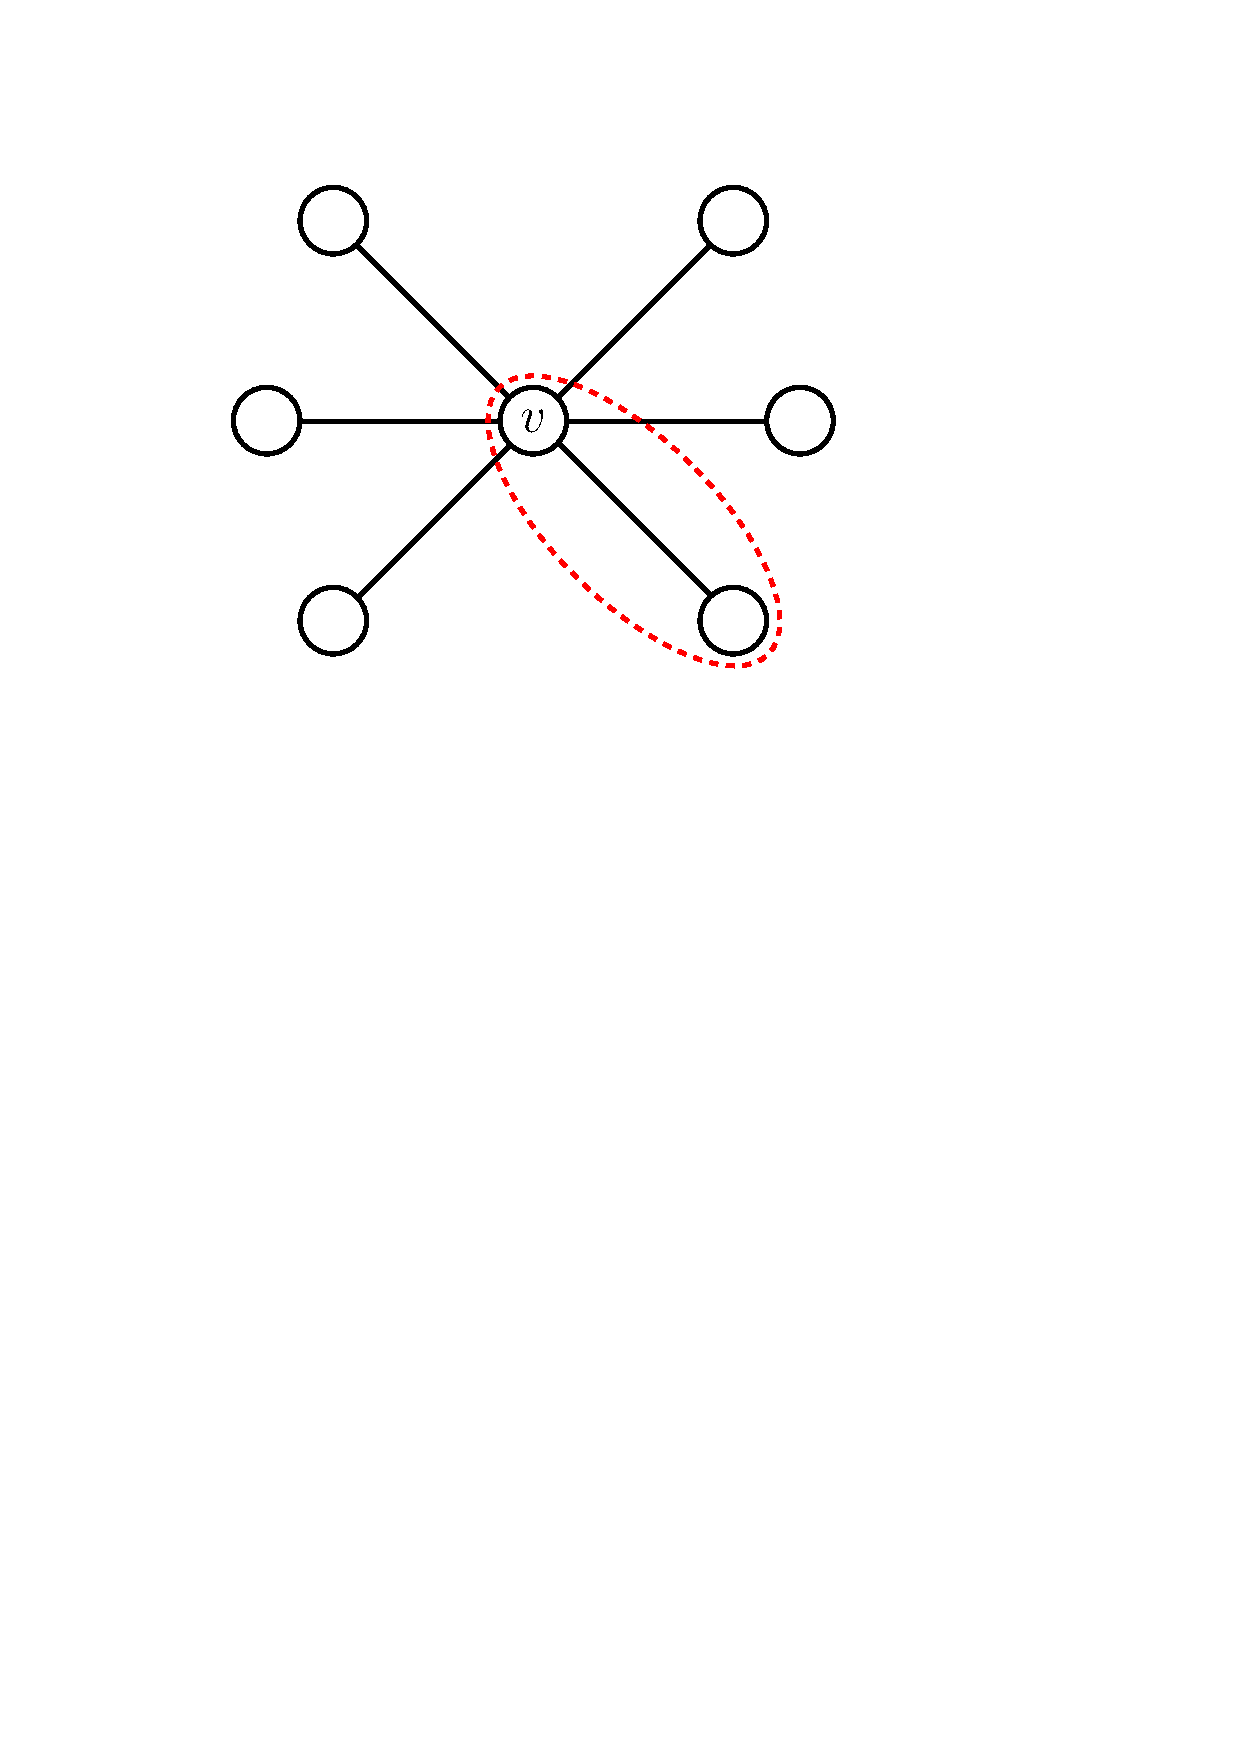
\includegraphics[scale=.5]{01_graph_theory/pics/graph_degree_handshaking-lemma.pdf}
}
\subfigure[directed graph, each edge is counted only once]{
	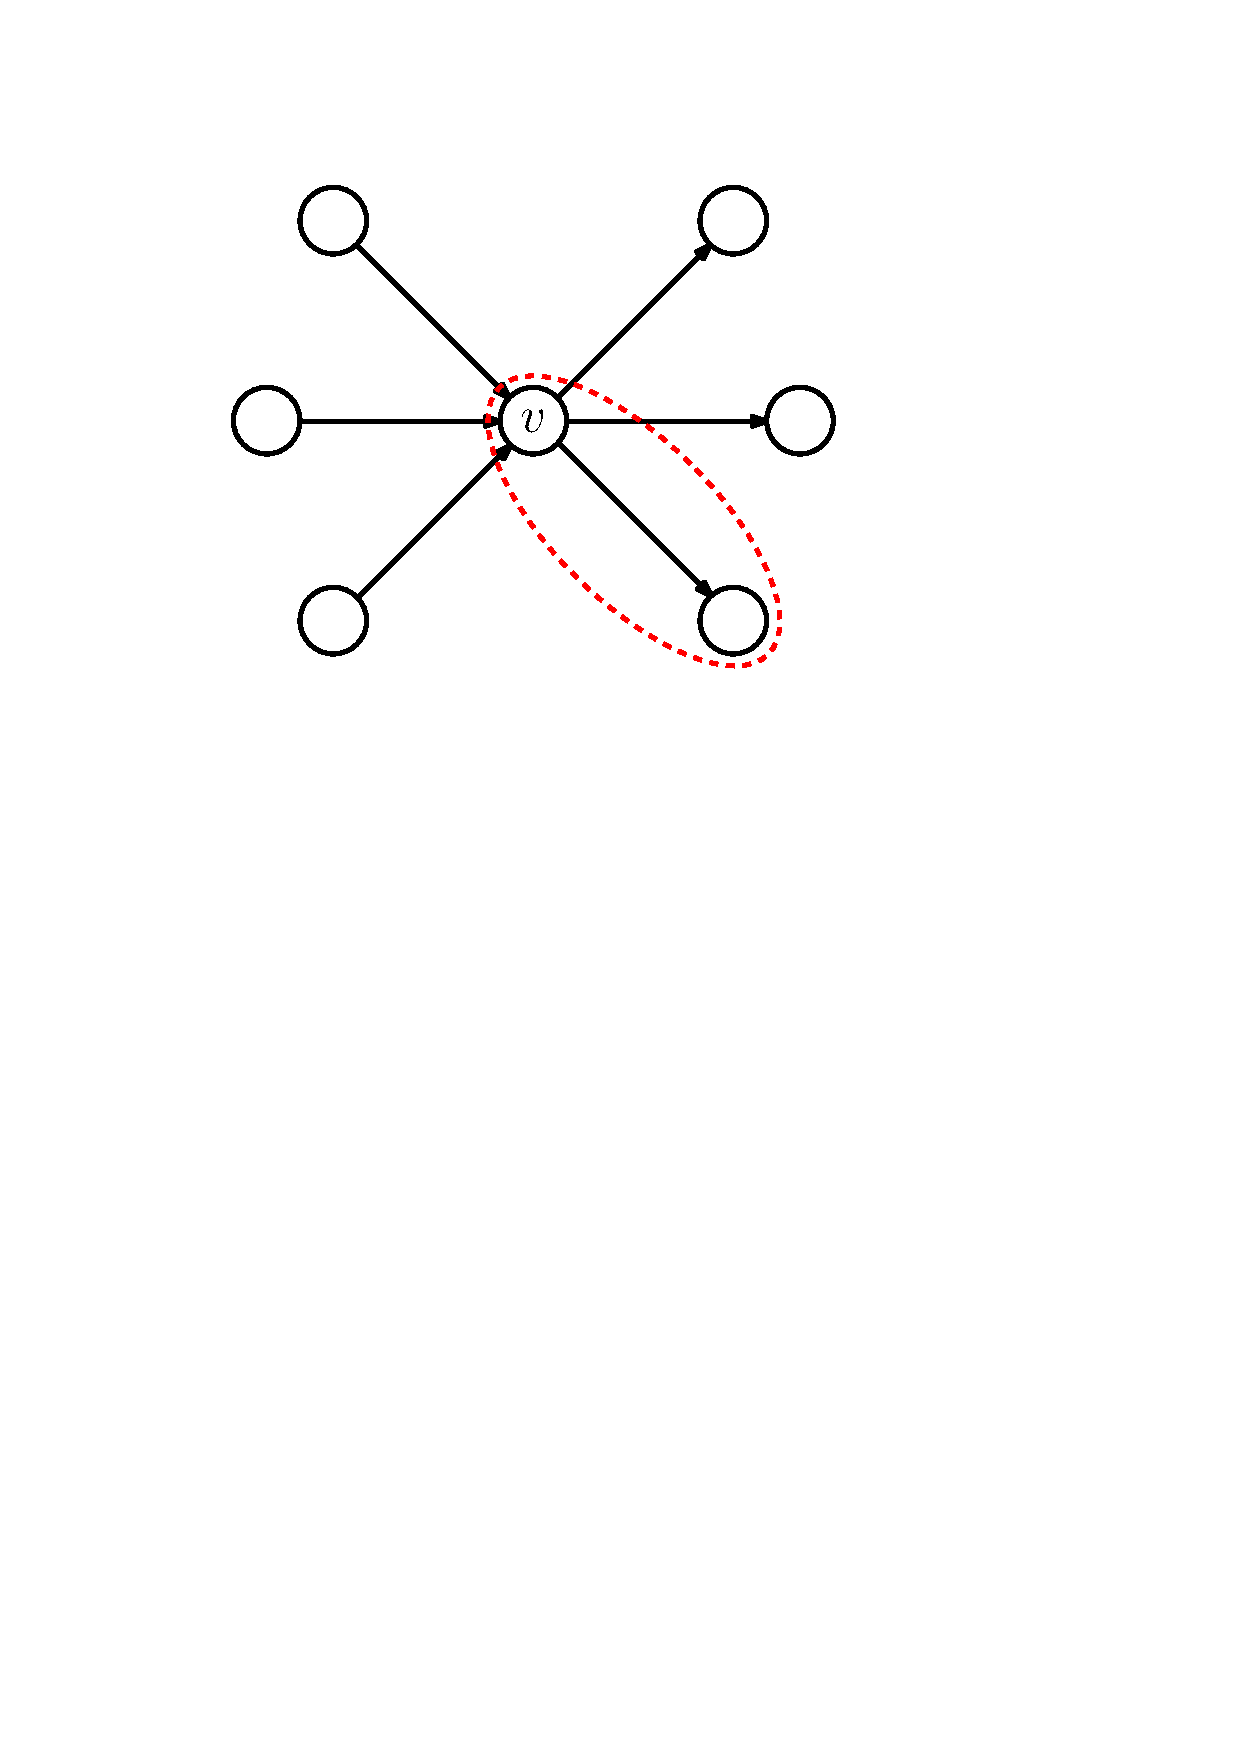
\includegraphics[scale=.5]{01_graph_theory/pics/directed-graph_degree_handshaking-lemma.pdf}
}
\caption{Hand Shaking Lemma in undirected and directed graphs}
\label{fig:hand_shaking_lemma}
\end{figure}
\FloatBarrier

\textbf{Example (Hypercube).} 
$G = (\{0,1\}^n, E)$

$vw \in E \Leftrightarrow \sum_{i=1}^{n} |v_i - w_i | = 1$ (only one switch in coordinates)

$v = v_1, v_2, \ldots , v_n$\\
$w = w_1, w_2, \ldots , w_n$

compute $a_0$ and $a_1$

$a_0 = 2^n$ \\
$a_1 = \frac{1}{2} \sum_{v \in V} d(v) = 2^{n-1} * n$

$d(v) = n \Rightarrow $ regular Graph
\begin{figure}[htb]
\centering
\subfigure[1D-hypercube]{
	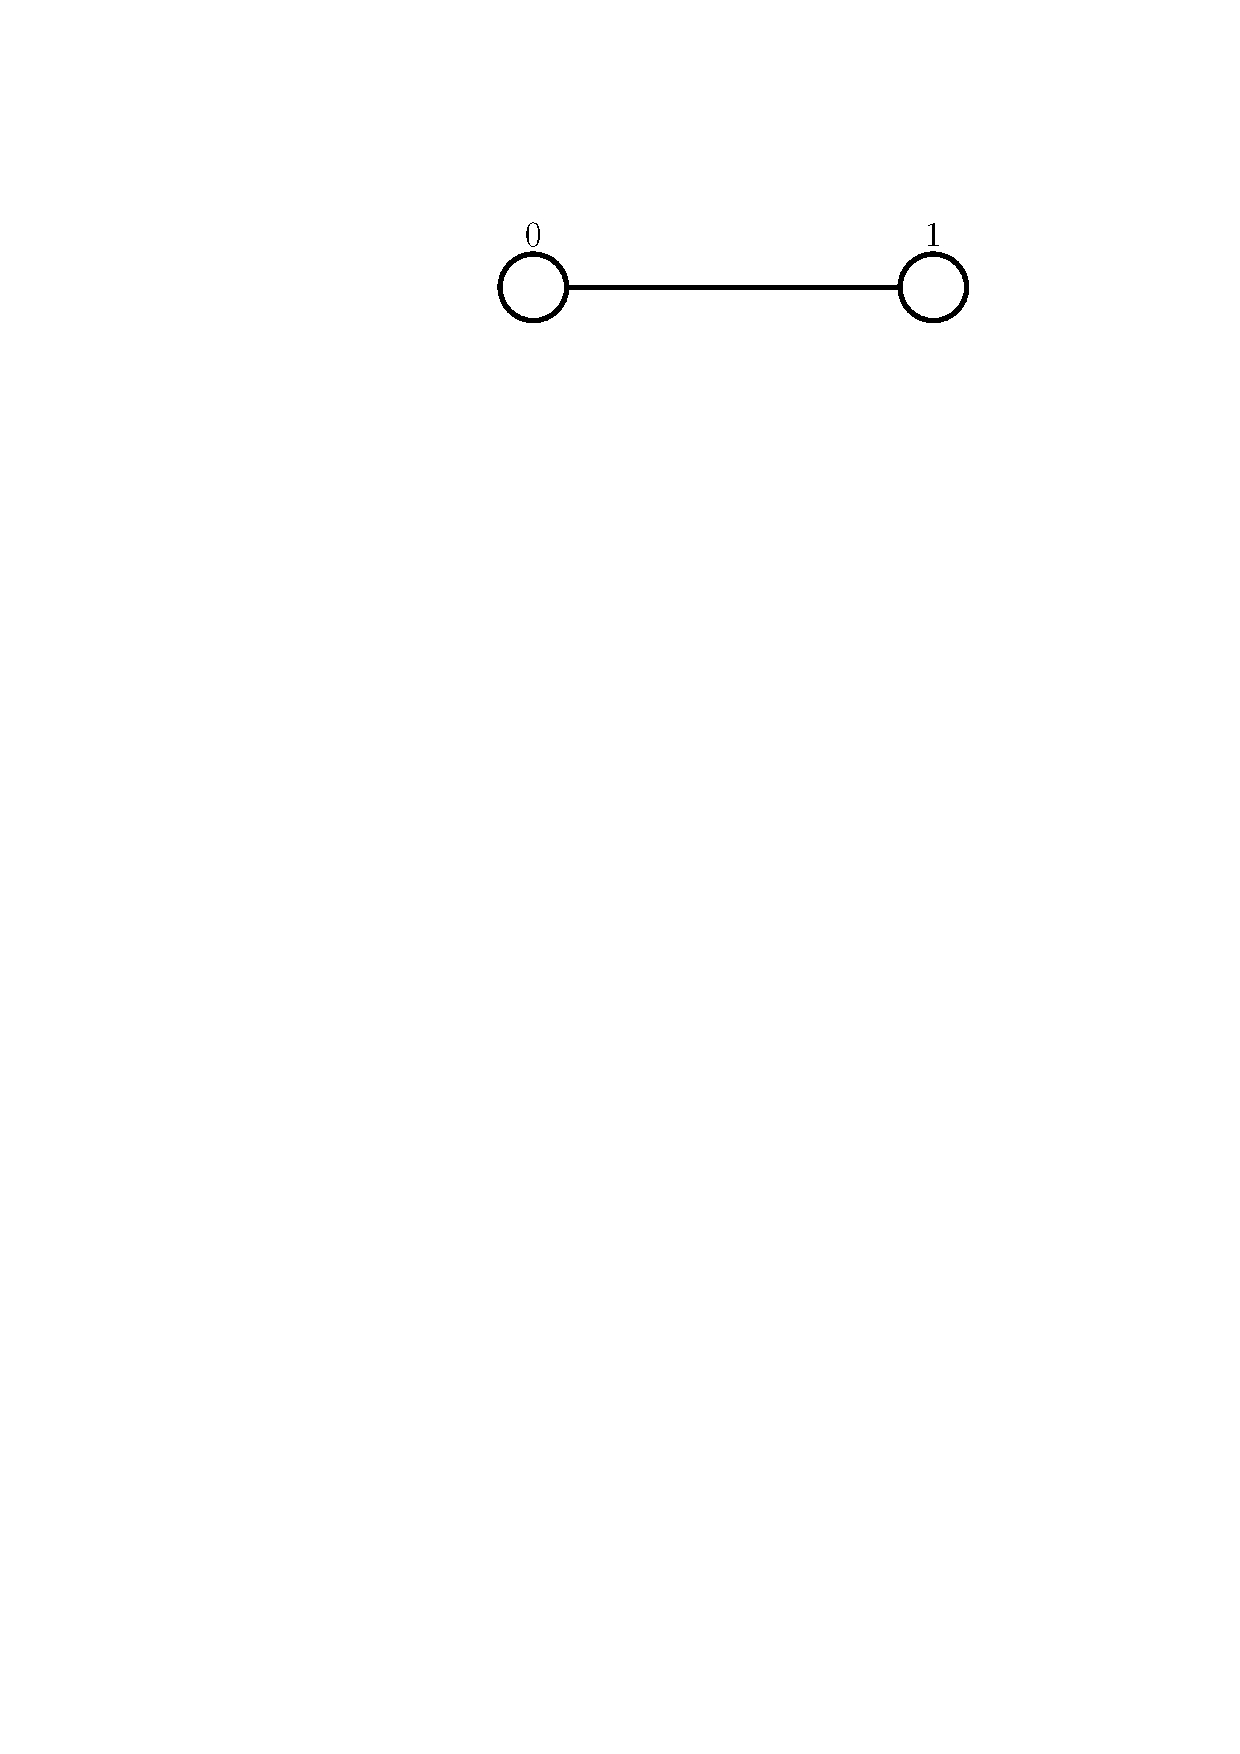
\includegraphics[scale=.4]{01_graph_theory/pics/1D-cube.pdf}
}
\subfigure[2D-hypercube]{
	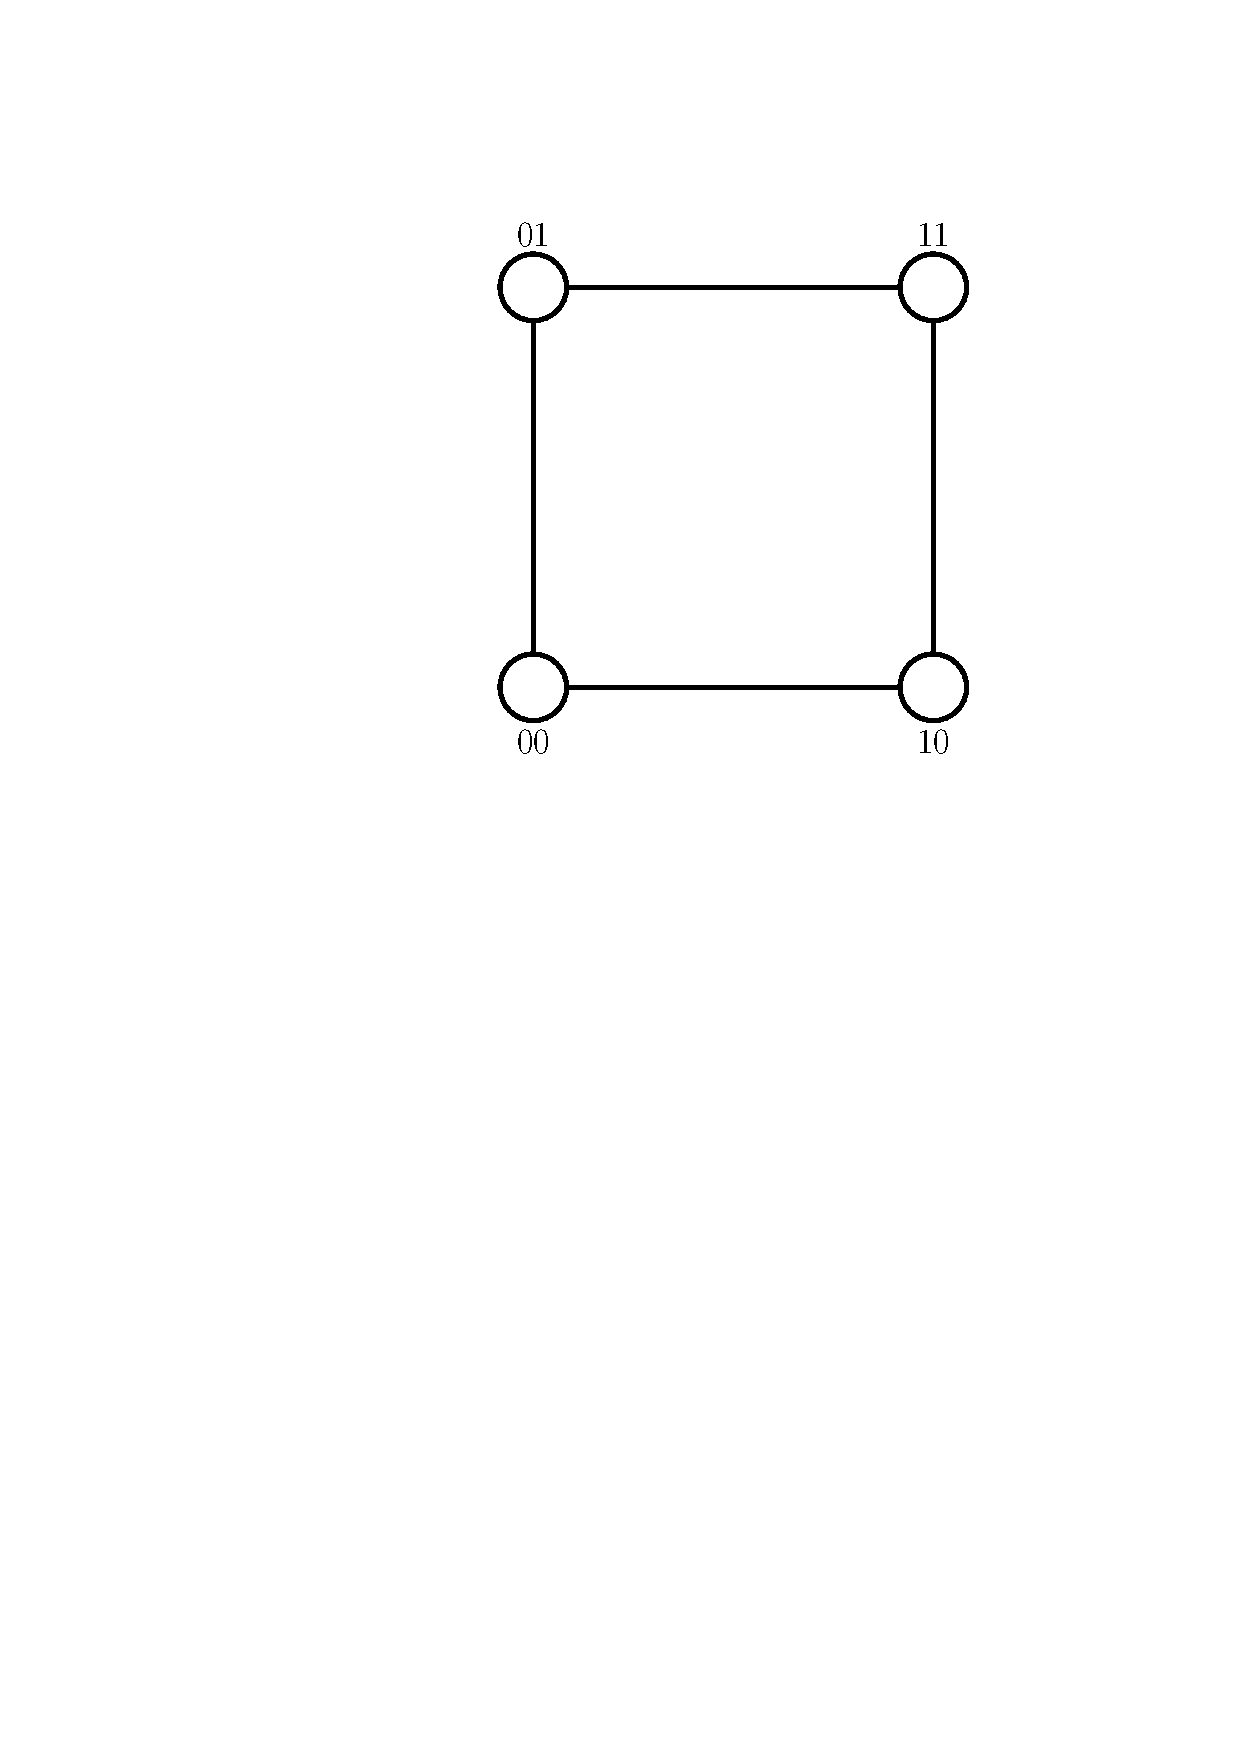
\includegraphics[scale=.4]{01_graph_theory/pics/2D-cube.pdf}
}
\subfigure[3D-hypercube]{
	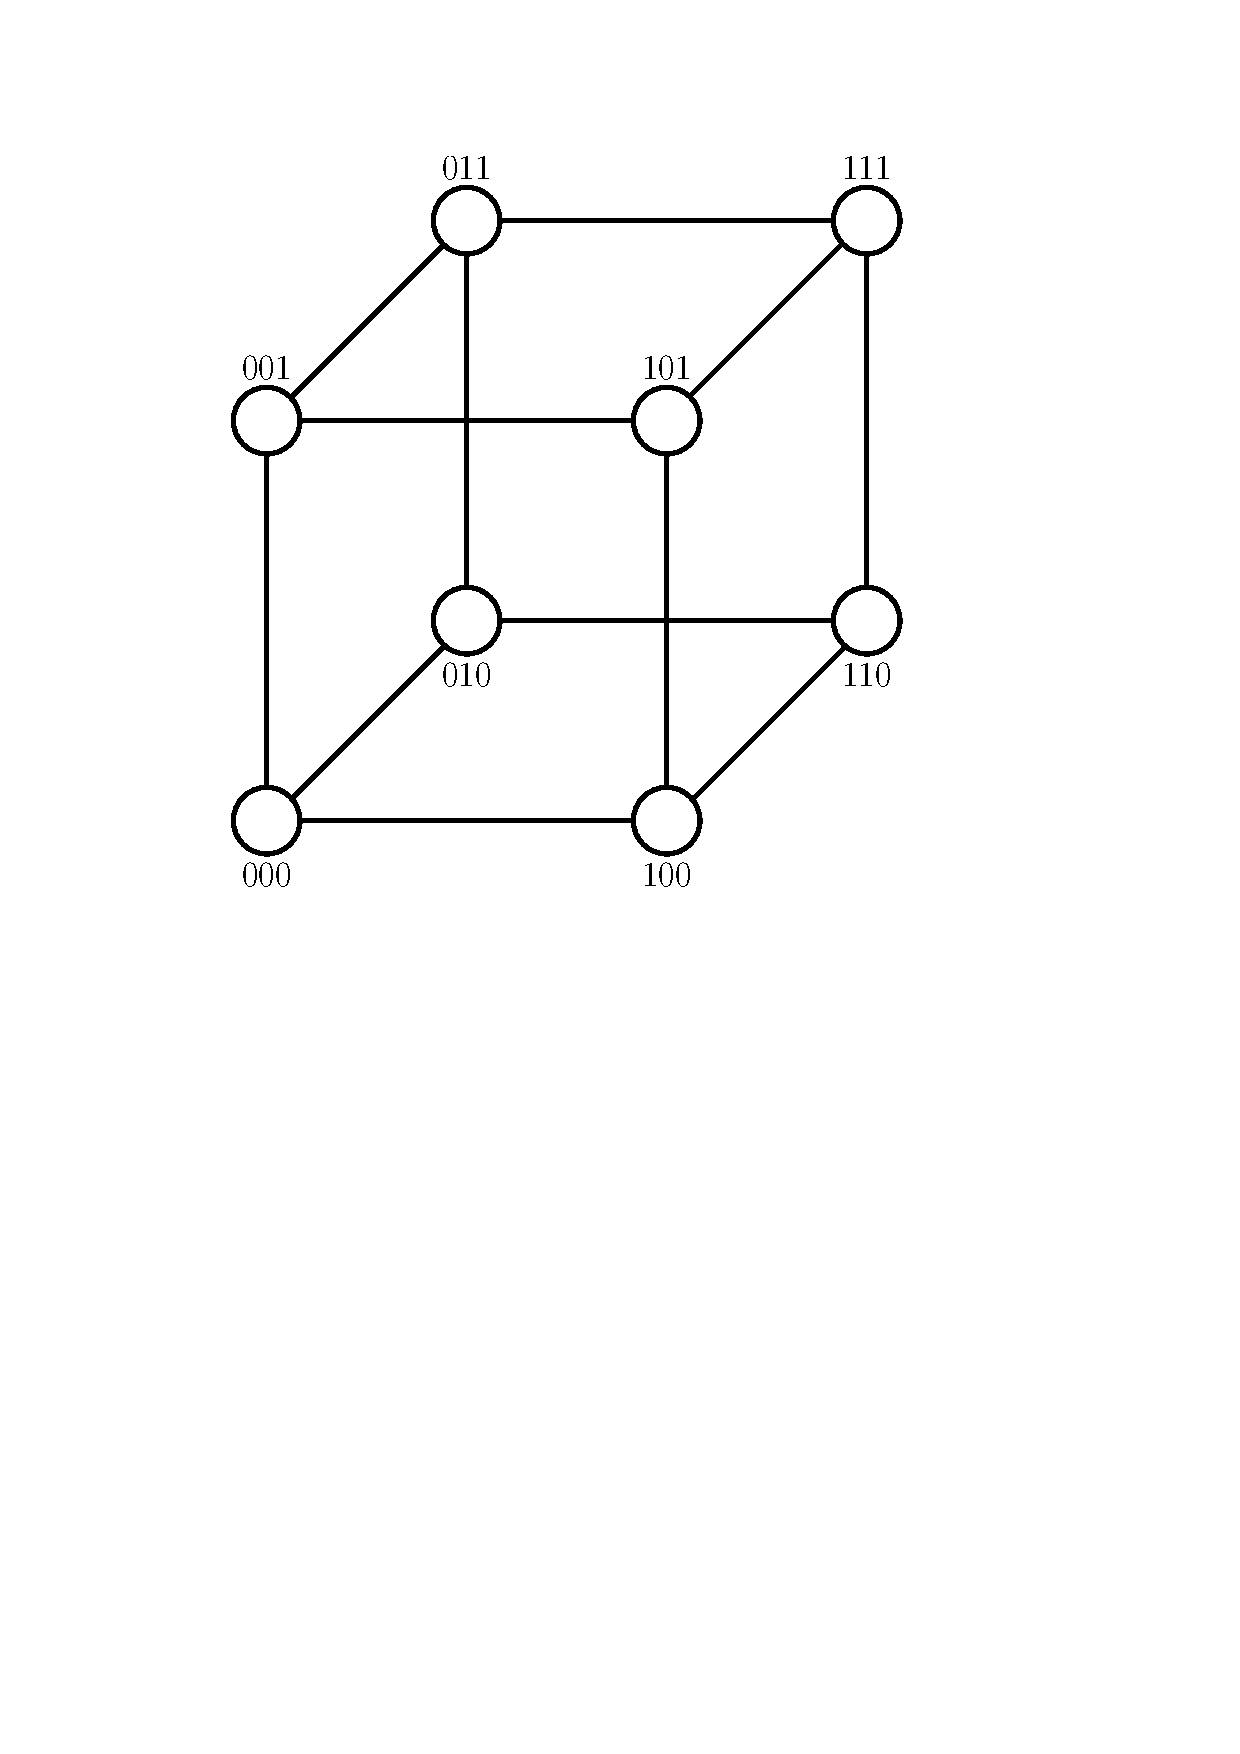
\includegraphics[scale=.4]{01_graph_theory/pics/3D-cube.pdf}
}
\caption{n-Hypercubes}
\end{figure}
\FloatBarrier

\begin{definition}
\index{adjacency}
\index{incidence}
Let $e=vw\in E$. Then we say that
\begin{compactitem}
\item $v$ and $w$ are \dt{adjacent} ($v\sim w$), and
\item $e$ and $v$ are \dt{incident} (as well as $e$ and $w$).
\end{compactitem}
\end{definition}

\begin{definition}
\index{adjacency!matrix}
Let $V=\{v_1,\ldots,v_n\}.$ The \dt{adjacency matrix} $A =
(a_{ij})_{i,j=1,\ldots,n}$ consists of entries
\[
  a_{ij} = \begin{cases}
    1 & v_i\sim v_j\text{ ($v_i$ and $v_j$ adjacent)} \\
    0 & v_i\not\sim v_j
  \end{cases}
\]
\end{definition}

\begin{figure}[htb]
\centering
\subfigure[adjacency $k = 1$]{
	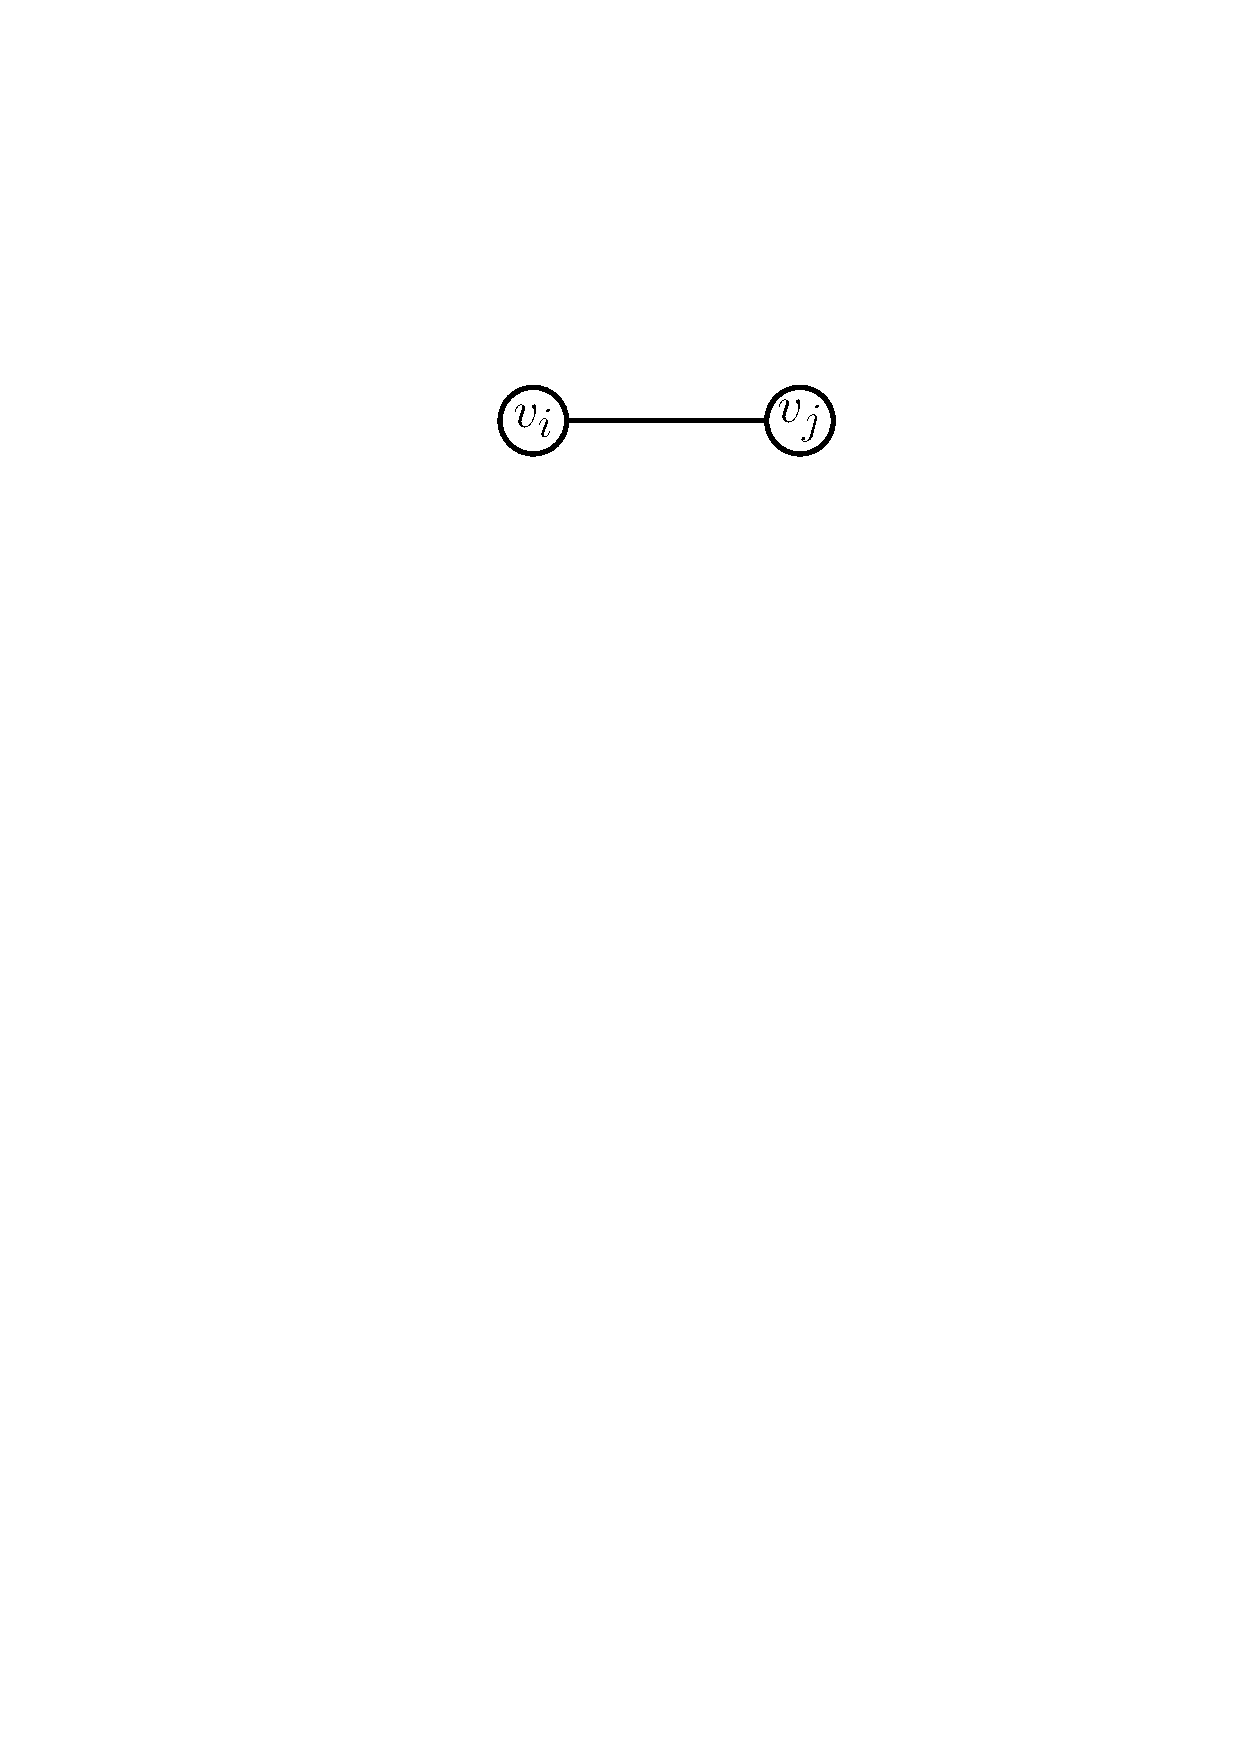
\includegraphics[scale=.5]{01_graph_theory/pics/adjacency_k-1.pdf}
}
\subfigure[adjacency $k = 2$]{
	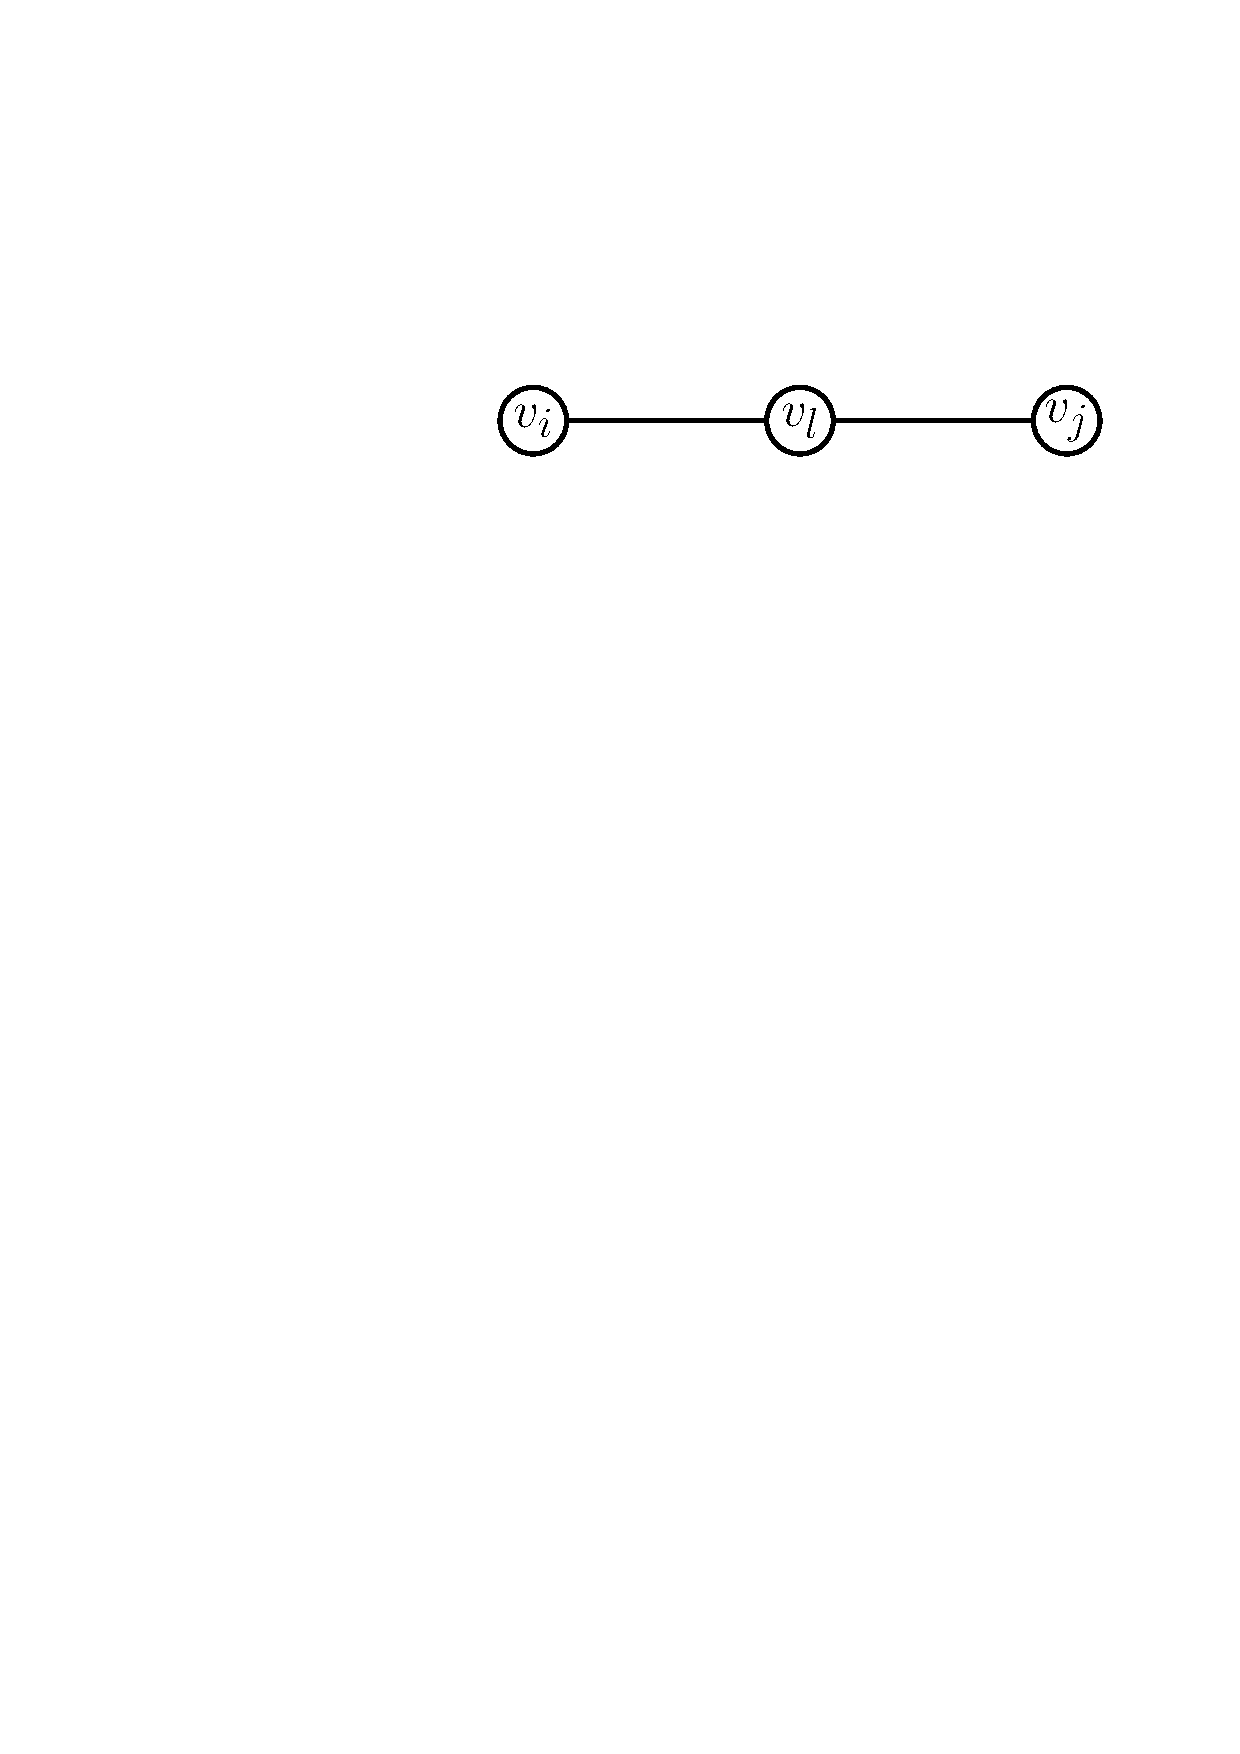
\includegraphics[scale=.5]{01_graph_theory/pics/adjacency_k-2.pdf}
}
\subfigure[adjacency via induction]{
	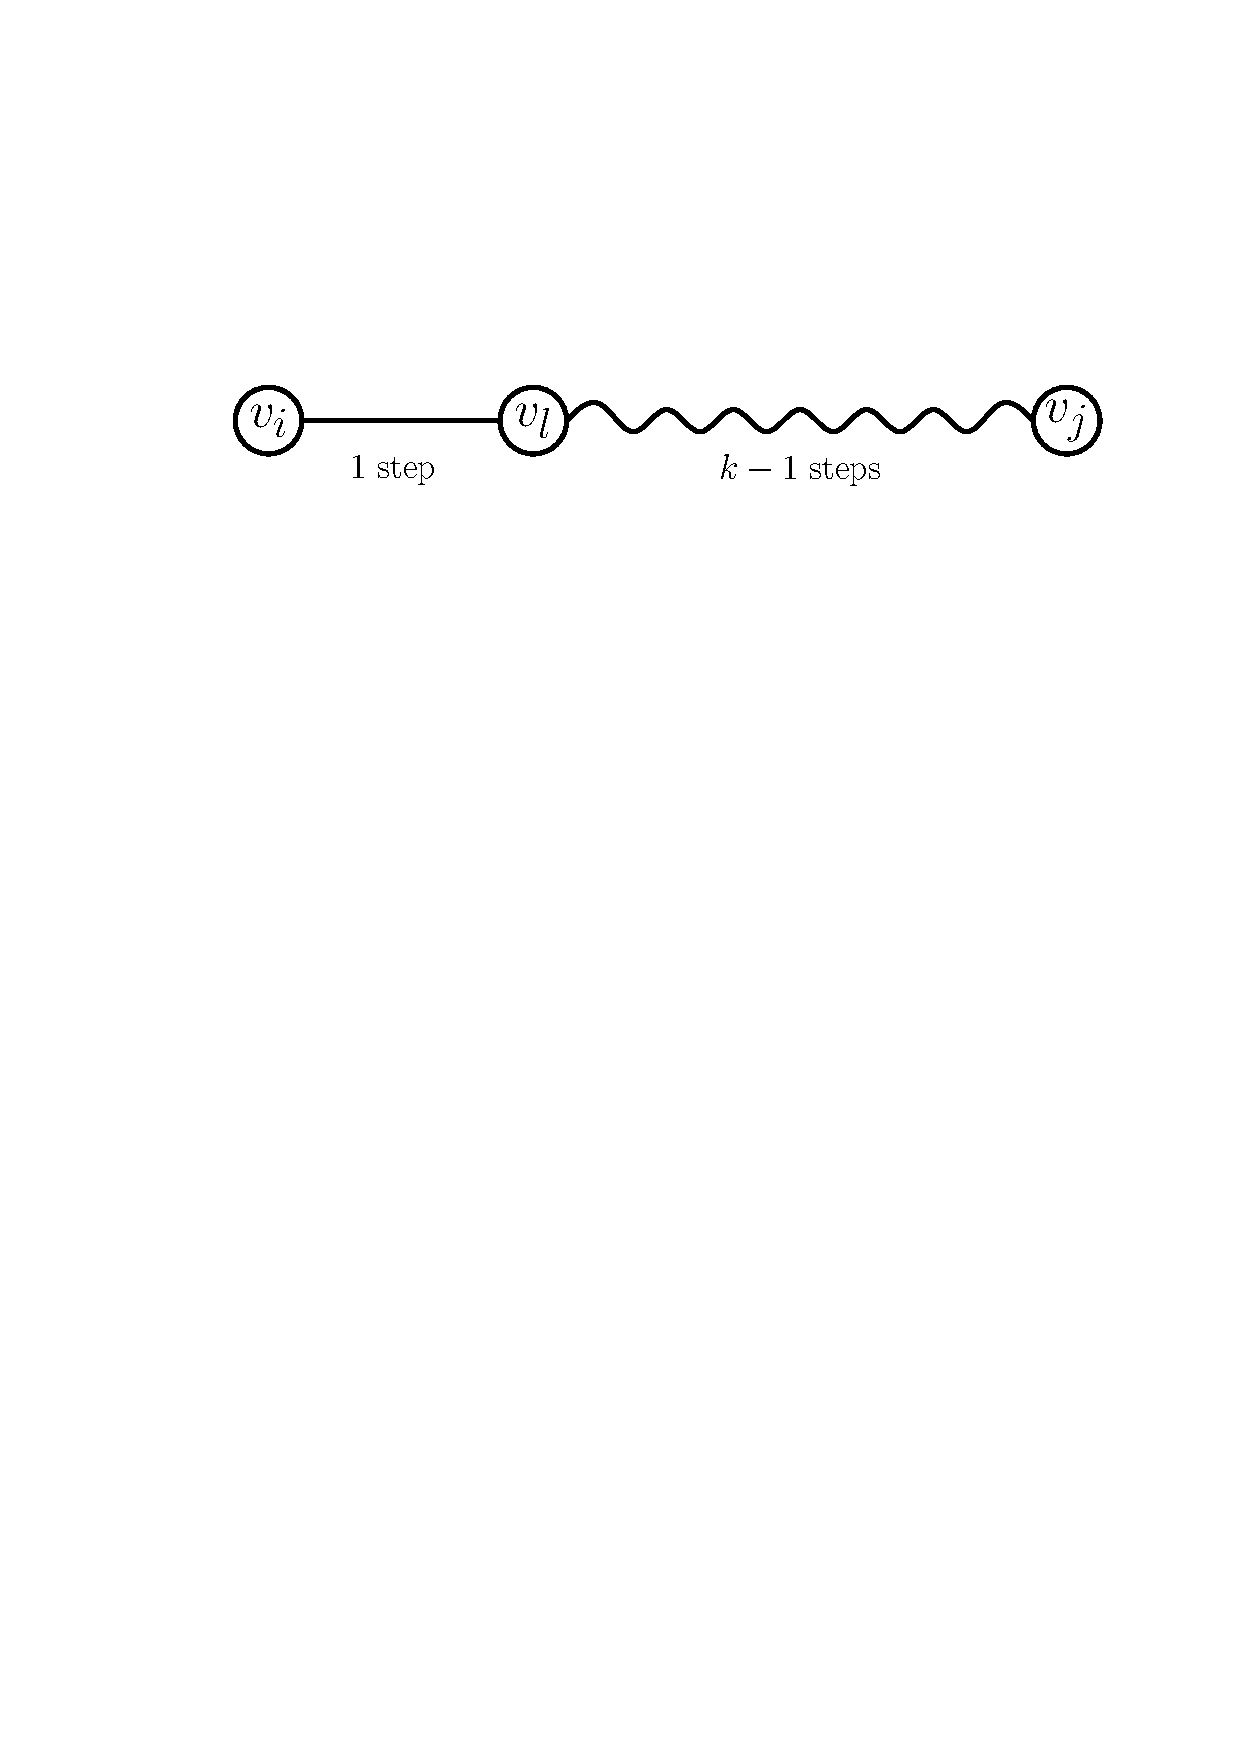
\includegraphics[scale=.5]{01_graph_theory/pics/adjacency_k-induction.pdf}
}
\caption{adjaceny}
\end{figure}
\FloatBarrier

\textbf{Remark.} If $G$ is undirected, $A$ is symmetric.

\textbf{Remark.} Consider
\begin{align*}
A^k &= (a_{ij}^{[k]})_{i,j=1,\ldots,n} = A\cdot A^{k-1} \\
a_{ij}^{[k]} &= \sum_{l=1}^n a_{il}^{\vphantom{[k-1]}}\cdot a_{lj}^{[k-1]}.
\end{align*}
The entries $a_{ij}^{[k]}$ of $A^k$ give the number of ways to get from $v_i$ to $v_j$ in exactly $k$ steps.

\begin{definition}
\index{walk}
A \dt{walk} in a graph $G$ is a sequence of edges, where successive edges have
a vertex in common. Edges can appear multiple times.
\end{definition}

\begin{figure}[htb]
\centering
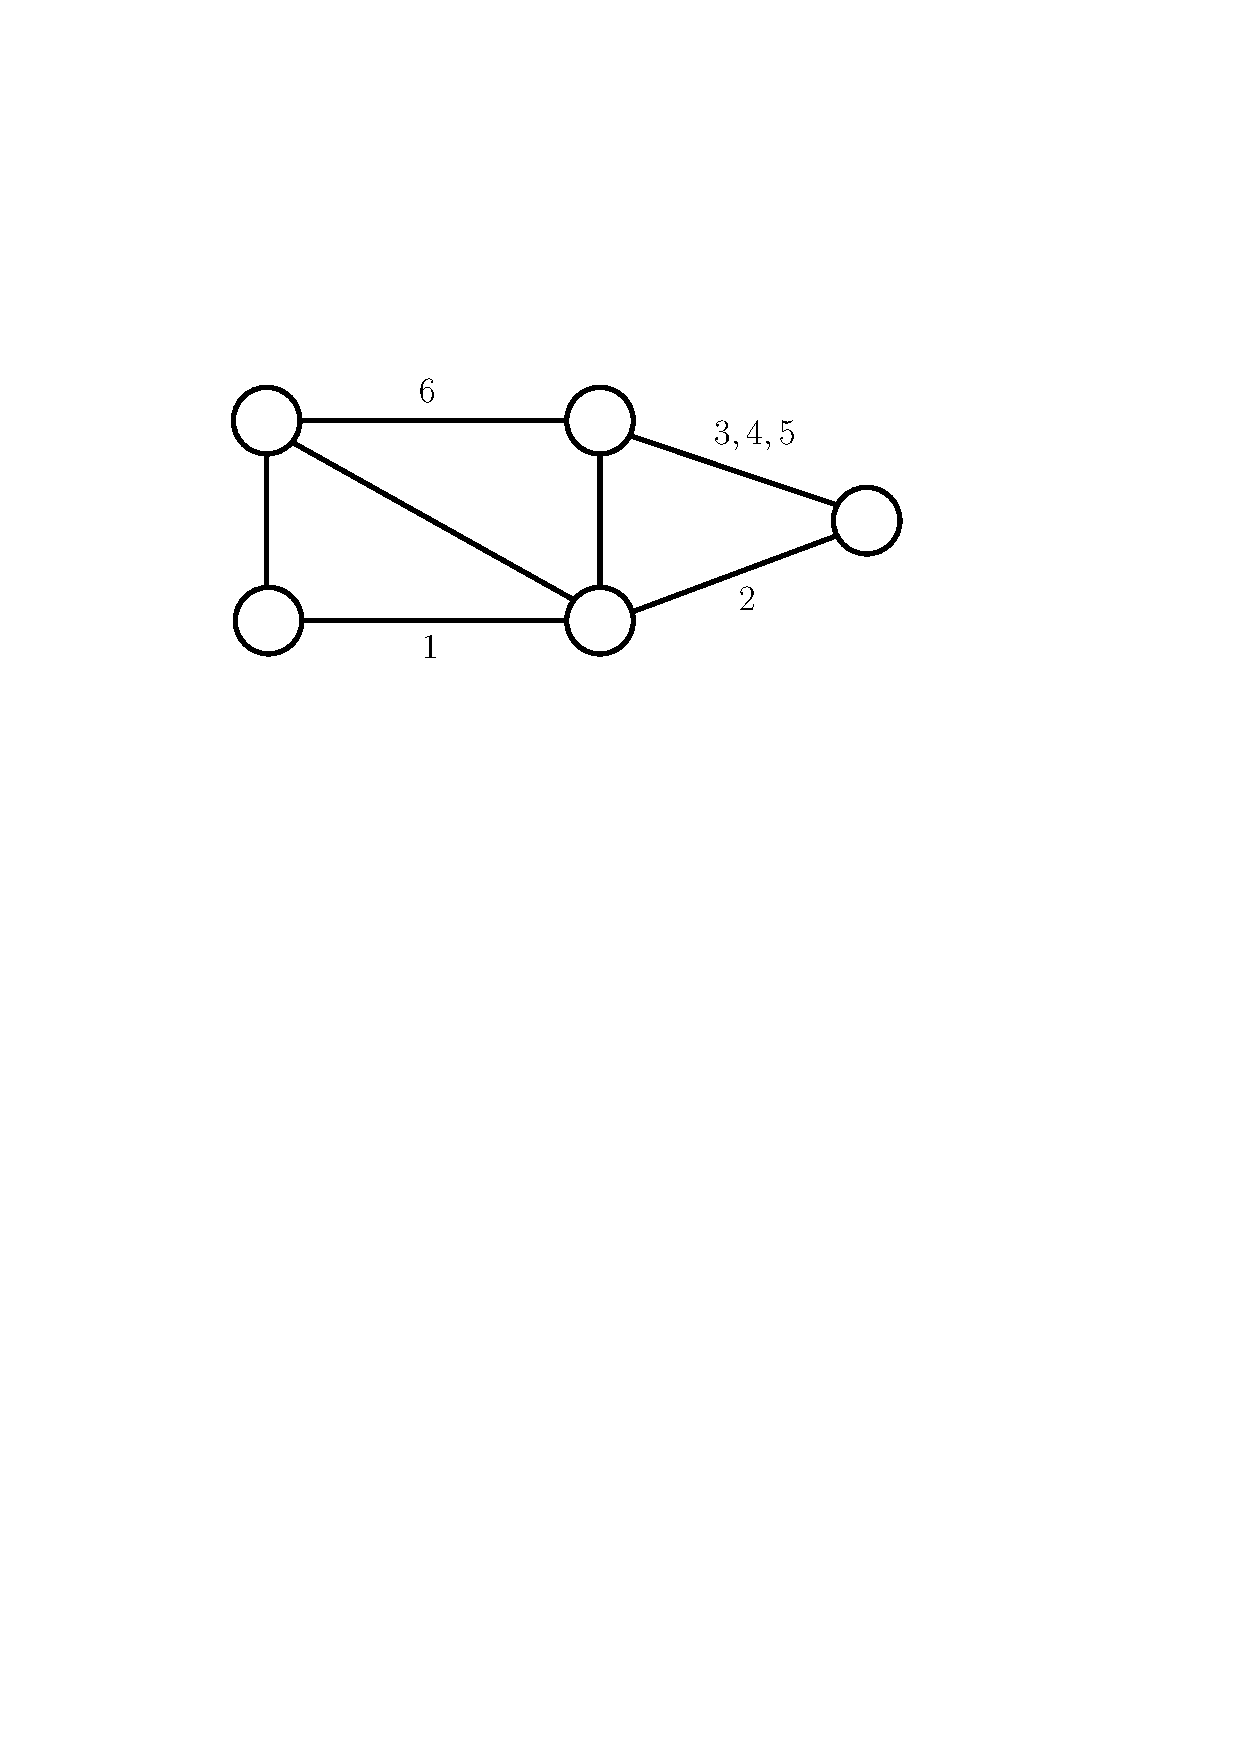
\includegraphics[scale=.5]{01_graph_theory/pics/walk.pdf}
\caption{Example of a walk through a graph}
\end{figure}
\FloatBarrier

\begin{definition}
\index{trail}
\index{circuit}
A \dt{trail} is a walk without repeated edges. A \dt{closed trail} or
\dt{circuit} starts and ends at the same vertex.
\end{definition}

\begin{definition}
\index{subgraph}
Let $G=(V,E)$. $H=(V',E')$ is a \dt{subgraph} of $G$ ($H \leq G$) if
\begin{compactitem}
\item $H$ is a graph,
\item $V' \subseteq V$, and
\item $E' \subseteq E$.
\end{compactitem}
$E'$ only contains edges between vertices in $V'$, this is implied by the requirement that $H$ is a graph.
\end{definition}

\begin{definition}
\index{connectivity}
\index{relation!connectivity relation}
For undirected graphs, we define the \dt{connectivity relation} $\operatorname{R}$ as follows:
\[ v \operatorname{R} w \text{ ($v$ connected to $w$)} \iff \exists\text{ walk from $v$ to $w$}. \]
\end{definition}

Let
\[ C = \sum_{k=0}^L A^k = (c_{ij})\qquad L = \min(|E|, |V|-1) \]
where $c_{ij}$ gives the number of walks from $v_ii$ to $v_j$ of length $\leq
L$. Now $M = \operatorname{sgn} C$ shows us which vertices are connected.

We observe that
\begin{compactitem}
\item $\forall v\in V: v \operatorname{R} v$,
\item $\forall v,w\in V: v \operatorname{R} v \implies w \operatorname{R} v$, and
\item $\forall v,w,u\in V: v \operatorname{R} v \wedge w \operatorname{R} v \implies v \operatorname{R} u$.
\end{compactitem}
\index{relation!equivalence relation}
Thus $\operatorname{R}$ is an \emph{equivalence relation} on $V$.

As an equivalence relation, $\operatorname{R}$ induces a partition of V.
\begin{gather*}
V = V_1 \cup\cdots\cup V_k \\
V_i \cap V_k = \varnothing\quad i\neq j
\end{gather*}
\index{connected component}%
$V_i$ are the \dt{connected components} of $G$.

\begin{figure}[htb]
	\centering
	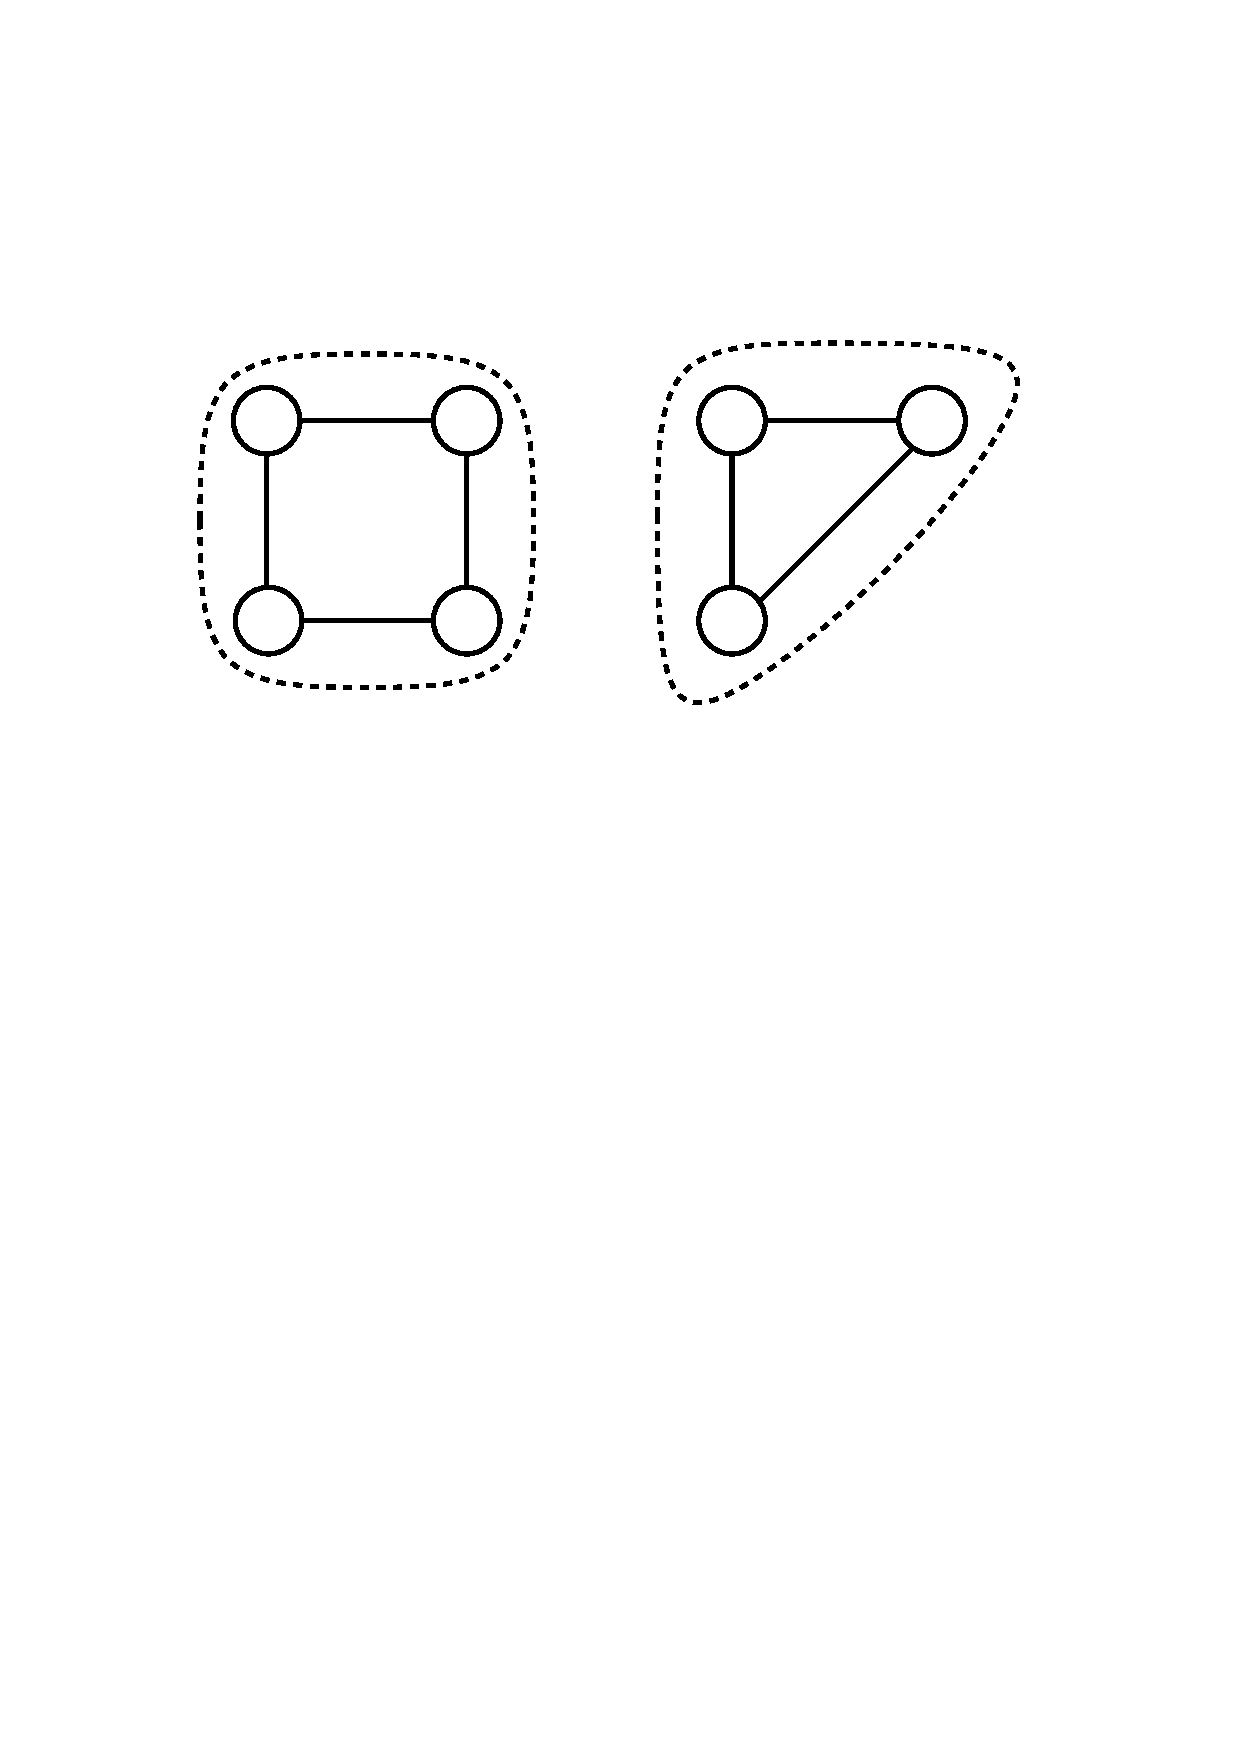
\includegraphics[scale=.5]{01_graph_theory/pics/components.pdf}
	\caption{Graph with 2 components}
\end{figure}
\FloatBarrier

\begin{definition}
\index{graph!connected}
$G$ is \dt{connected} if it has only one component. This means that $\forall v,w: v\operatorname{R} w$.
\end{definition}

\begin{definition}
\index{connected component}
$H\leq G$ is a \dt{connected component} of $G$ if $H$ is connected and $H$
is maximal with regard to the subgraph relation, i.\,e. no vertices or edges can
be added to $H$ so that is still connected: $\nexists H': H < H' \leq G, H'\text{ connected}.$
\end{definition}

\begin{definition}
\index{connectivity}
\index{relation!connectivity relation}
For directed graphs, we define the \dt{connectivity relation} $\operatorname{S}$ as follows:
\begin{align*}
v \operatorname{R} w \text{ ($v$ connected to $w$)} \iff \null
&\text{$\exists$ walk from $v$ to $w$\quad\emph{and}} \\
&\text{$\exists$ walk from $w$ to $v$.}
\end{align*}
Like $\operatorname{R}$, $\operatorname{S}$ is an equivalence relation.
\end{definition}

\begin{definition}
\index{graph!connected!strongly}
$G$ is \dt{strongly connected} $\iff \forall v,w\in V: v \operatorname{S} w$.
\end{definition}

\begin{definition}
\index{connected component!strongly}
$H\leq G$ is a \dt{strongly connected component} of $G$ if $H$ is maximal strongly connected.
\end{definition}

\begin{figure}[htb]
	\centering
	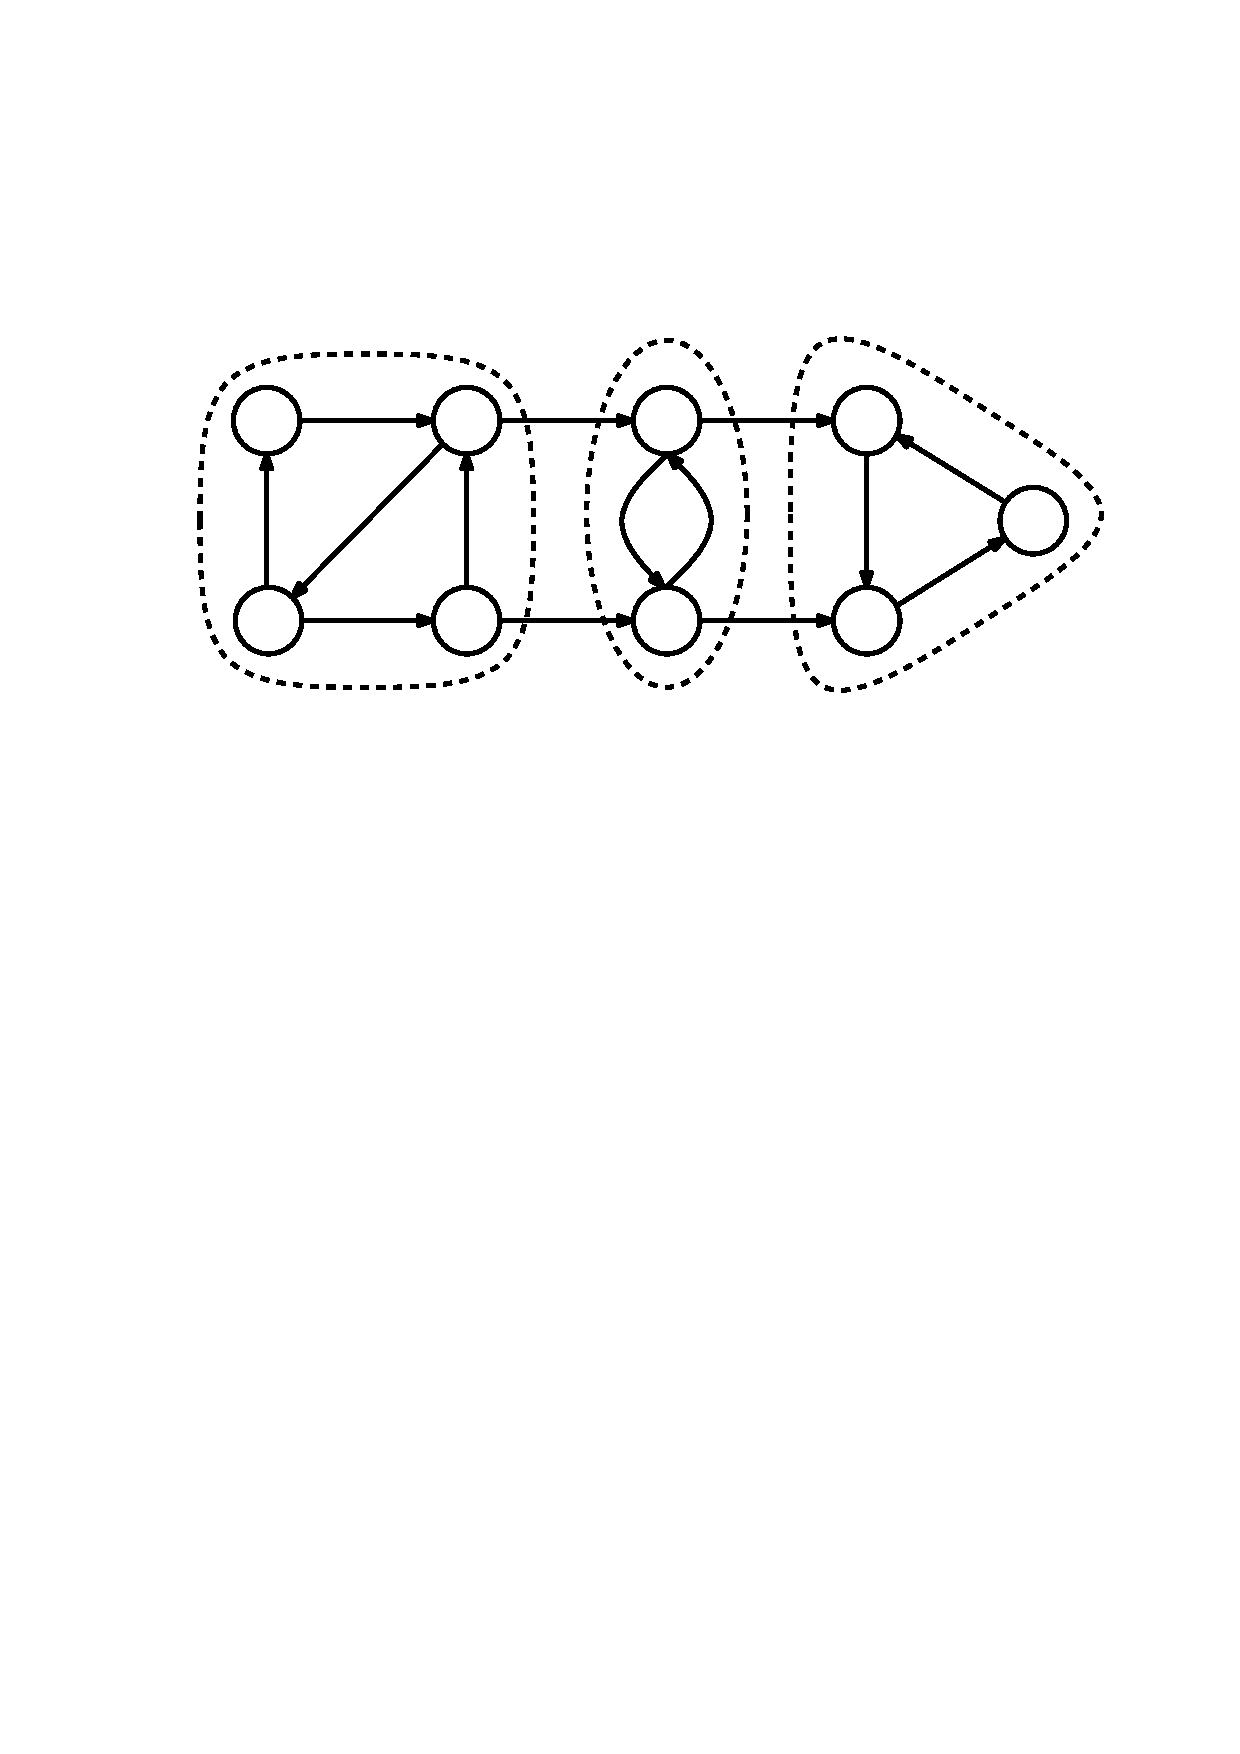
\includegraphics[scale=.5]{01_graph_theory/pics/strongly-connected_component.pdf}
	\caption{graph with 3 strongly connected components}
\end{figure}
\FloatBarrier


%%%  04.10.2013  %%%
%%%  VO 02

\begin{definition}
\strut\lecturedate{2013-10-04}%
\index{shadow}
Let $G$ be a directed graph. The \dt{shadow} $H$ of $G$ is the undirected graph
that results when we ignore edge directions on $G$.
\end{definition}

\begin{definition}
\index{graph!connected!weakly}
$G$ is \dt{weakly connected} if its shadow $H$ is connected.
\end{definition}

\begin{definition}
\def\Gr{\ensuremath{G_\text{R}}}
\def\Vr{\ensuremath{V_\text{R}}}
\def\Er{\ensuremath{E_\text{R}}}
Let $G=(V,E)$ be a directed graph. Let
\[ K_1=\{v_1,\ldots\},K_2,\ldots,K_M \]
be the strongly connected components of $G$. Let $\Gr=(\Vr,\Er)$ with
\begin{align*}
\Vr &= \{K_1,\ldots,K_M\} \\
\Er &= \left\{(K_i,K_j) \mid \exists v\in V(K_i)\,\exists w\in V(K_j): (v,w)\in E\right\}.
\end{align*}
\index{reduction}%
Then we call $\Gr$ the \dt{reduction} of $G$.
\end{definition}

\textbf{Remark.} $G_\text{R}$ is always acyclic.

% strongly connected components
\begin{figure}[htb]
\resizebox{\textwidth}{!}{
\subfigure[directed Graph $G$]
{
	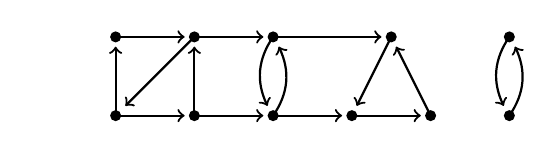
\begin{tikzpicture}
	\node at (0,0) {};
	\node (k1) at (1,0) {};
	\node (k2) at (2,0) {};
	\node (k3) at (2,1) {};
	\node (k4) at (1,1) {};

	\node (k5) at (3,0) {};
	\node (k6) at (3,1) {};

	\node (k7) at (4,0) {};
	\node (k8) at (5,0) {};
	\node (k9) at (4.5,1) {};

	\node (k10) at (6,0) {};
	\node (k11) at (6,1) {};

	\foreach \i in {1,...,11}
	{
		\fill (k\i) circle [radius=2pt];
	};

	\foreach \i / \j in {
	1/2, 2/3, 3/1, 4/3, 1/4,
	7/8, 8/9, 9/7,
	2/5, 3/6,
	5/7,
	6/9}
	{
		\path (k\i.center) edge[->, thick] (k\j);
	};
	\foreach \i / \j in {
	5/6, 6/5,
	10/11, 11/10}
	{
		\path (k\i.center) edge[->, thick, bend right] (k\j);
	};

	\end{tikzpicture}
}
\subfigure[shadow $H$ of Graph $G$]
{
	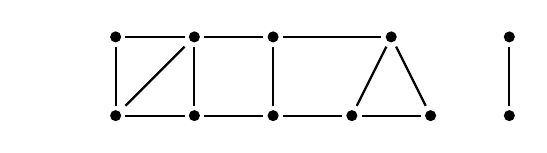
\begin{tikzpicture}
	\node at (0,0) {};
	\node (k1) at (1,0) {};
	\node (k2) at (2,0) {};
	\node (k3) at (2,1) {};
	\node (k4) at (1,1) {};

	\node (k5) at (3,0) {};
	\node (k6) at (3,1) {};

	\node (k7) at (4,0) {};
	\node (k8) at (5,0) {};
	\node (k9) at (4.5,1) {};

	\node (k10) at (6,0) {};
	\node (k11) at (6,1) {};

	\foreach \i in {1,...,11}
	{
		\fill (k\i) circle [radius=2pt];
	};

	\foreach \i / \j in {
	1/2, 2/3, 3/1, 4/3, 1/4,
	7/8, 8/9, 9/7,
	2/5, 3/6,
	5/7,
	6/9,
	5/6, 6/5,
	10/11, 11/10}
	{
		\path (k\i) edge[thick] (k\j);
	};
	\end{tikzpicture}
}}
\resizebox{\textwidth}{!}{
\subfigure[strongly connected components of $G$]
{
	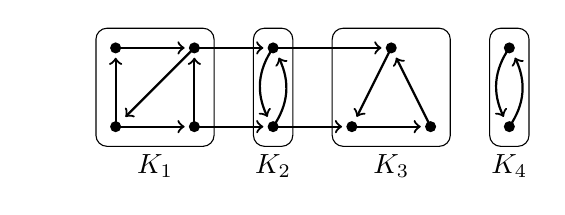
\begin{tikzpicture}
	\node at (0,0) {};
	\node (k1) at (1,0) {};
	\node (k2) at (2,0) {};
	\node (k3) at (2,1) {};
	\node (k4) at (1,1) {};

	\node (k5) at (3,0) {};
	\node (k6) at (3,1) {};

	\node (k7) at (4,0) {};
	\node (k8) at (5,0) {};
	\node (k9) at (4.5,1) {};

	\node (k10) at (6,0) {};
	\node (k11) at (6,1) {};

	\foreach \i in {1,...,11}
	{
		\fill (k\i) circle [radius=2pt];
	};

	\foreach \i / \j in {
	1/2, 2/3, 3/1, 4/3, 1/4,
	7/8, 8/9, 9/7,
	2/5, 3/6,
	5/7,
	6/9}
	{
		\path (k\i.center) edge[->, thick] (k\j);
	};
	\foreach \i / \j in {
	5/6, 6/5,
	10/11, 11/10}
	{
		\path (k\i.center) edge[->, thick, bend right] (k\j);
	};

	\draw[rounded corners] (0.75, -0.25) rectangle (2.25, 1.25);
	\draw[rounded corners] (2.75, -0.25) rectangle (3.25, 1.25);
	\draw[rounded corners] (3.75, -0.25) rectangle (5.25, 1.25);
	\draw[rounded corners] (5.75, -0.25) rectangle (6.25, 1.25);

	\node at (1.5, -0.5) {$K_1$};
	\node at (3.0, -0.5) {$K_2$};
	\node at (4.5, -0.5) {$K_3$};
	\node at (6.0, -0.5) {$K_4$};
	\end{tikzpicture}
}
\subfigure[reduction $G_R$ of Graph $G$]
{
	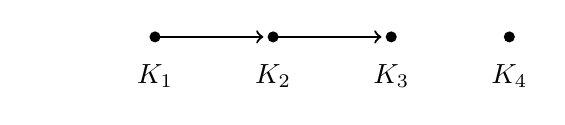
\begin{tikzpicture}
	\node at (0,0) {};
	\node (k1) at (1.5, 0) {};
	\node (k2) at (3.0, 0) {};
	\node (k3) at (4.5, 0) {};
	\node (k4) at (6.0, 0) {};

	\node at (1.5, -0.5) {$K_1$};
	\node at (3.0, -0.5) {$K_2$};
	\node at (4.5, -0.5) {$K_3$};
	\node at (6.0, -0.5) {$K_4$};

	\foreach \i in {1,...,4}
	{
		\fill (k\i) circle [radius=2pt];
	};
	\foreach \i / \j in {1/2, 2/3}
	{
		\path (k\i.center) edge[->, thick] (k\j);
	};
	\end{tikzpicture}
}}
\caption{Graphs}
\end{figure}





\begin{definition}
\index{node base}
Let $G$ be a directed graph. $B$ is a \dt{node base} of $G$ if:
\begin{compactitem}
\item $B\subseteq V$,
\item $\forall v\in V\,\exists w\in B: w \operatorname{S} v$, and
\item $B$ minimal w.\,r.\,t. $\subseteq$.
\end{compactitem}
\end{definition}

\index{node base}
\textbf{Remark.} The node base of $G$ can easily be constructed from a node
base of $G_\text{R}$. Let $\{K_1,\ldots,K_L\}\subseteq V_\text{R}$ be a node
base of $G_\text{R}$. Then
\[ \left\{\{b_1,\ldots,b_l\mid b_i\in V(K_i)\}\right\} \]
is the set of all node bases of $G$.

\index{node base}
$G_\text{R}$ has a single unique node base.

\index{node base}
\textbf{Remark.} The node base of $G_\text{R}$ (or acyclic graphs in general) is
\[ \{K\in V_\text{R}\mid d_{G_\text{R}}^{-}(K) = 0\}. \]




%%%  04.10.2013  %%%
%%%  VO 02
\section{Trees and Forests}

\begin{definition}
\index{forest}
A \dt{forest} is an undirected acyclic graph.
\end{definition}

\begin{definition}
\index{tree}
A \dt{tree} is a connected forest.
\end{definition}

\begin{definition}
\index{tree!rooted}
\index{root}
A \dt{rooted tree} is a tree with one special node designated as the \dt{root}.
\end{definition}

\begin{definition}
\index{tree!plane}
A \dt{plane tree} is a tree embedded into the plane, i.\,e. the order of
children matters. Two trees may be isomorphic, but not equivalent when regarded
as plane trees.
\end{definition}

In Computer Science, trees are often plane and rooted, e.\,g.\ binary search trees.

\begin{definition}
\index{isomorphism}
Two graphs $G$ and $H$ are \dt{isomorphic} ($G \cong H$) if there is a function
\[ \varphi: V(G)\mapsto V(H)\quad\text{$\varphi$ bijective} \]
so that
\[ vw \in E(G) \iff \varphi(v)\varphi(w) \in E(H). \]
\end{definition}

\begin{definition}
\index{leaf}
A \dt{leaf} is a node with degree 1. 
\end{definition}

\textbf{Lemma.}
A non rooted tree $T$ has at least 2 leaves. \\
$|V(T)| \geq 2$

\textbf{Proof.} \TODO{add images} \\
\begin{compactitem}
	\item T of size 2
	\item T of at least 3 nodes, $|V(T)| \geq 3$
	\begin{compactitem}
		\item Case 1:\\
			$|V(T)| = k+1 \Rightarrow |V(T)| = k$ \\
			$\Rightarrow_{imp} T'$ has 2 leaves $\Rightarrow T$ has at least 2 leaves
		\item Case 2: \\
			first node is no leaf, $T'$ and $T''$ each have at least 2 leaves each

	\end{compactitem}
\end{compactitem}


\begin{definition}
\index{bridge}
A \dt{bridge} is an edge whose removal would increase the number of connected components.
\end{definition}


\textbf{Theorem.} The following statements are equivalent:
\begin{compactenum}[(1)]
  \item $T$ is a tree.
  \item $\forall v,w\in V(T)$ $\exists$ unique path from $v$ to $w$
  \item $T$ connected, $|V(T)|=|E(T)|+1$
  \item $T$ minimal connected (every edge is a bridge)
  \item $T$ maximal acyclic
\end{compactenum}
\null\par

\textbf{Proof of 1. $\implies$ 3.} \\
induction on $n = \alpha_0=|V(T)|$

\begin{tabular}{l l}
	$n = 1:$	& trivial, $\cdot$ \\
	$n \rightarrow n+1:$	& Choose leaf $v$ of $T$, $T' = T \backslash \{v\}$ \\
							 &	
	$\begin{array}{ll}
	|V(T')| = |E(T')| + 1 \\
		|V(T')+1 = |E(T')+1 +1 \\
		substitution	& |V(T)| = |V(T')| +1 \\
			& |E(T)| = |E(T')| +1 \\
		|V(T)| = |E(T)| + 1
	\end{array}$
\end{tabular}

\subsection{Spanning Subgraphs}

\begin{definition}
\index{spanning forest}
\index{spanning tree}
Let $G=(V,E)$ be an undirected graph. $F$ is a \dt{spanning forest} of $G$ if and only if:
\begin{compactitem}
  \item $V(F) = V(G)$, $E(F)\subseteq E(G)$,
  \item $F$ is a forest, and
  \item $F$ has the same connected components as $G$.
\end{compactitem}
If $F$ is connected, we call it a \dt{spanning tree}.
\end{definition}

\textbf{Example introducing matrix-tree theorem}\\

% Graph G and all possible spanning trees
\begin{figure}[htb]
\centering
\subfigure
{
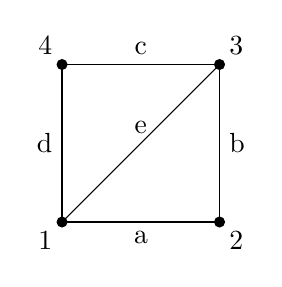
\begin{tikzpicture}[scale=2]

\node (n1) at (0,0) {};
\node (n2) at (1,0) {};
\node (n3) at (1,1) {};
\node (n4) at (0,1) {};

\draw (n1) node[anchor=north east] {$1$};
\draw (n2) node[anchor=north west] {$2$};
\draw (n3) node[anchor=south west] {$3$};
\draw (n4) node[anchor=south east] {$4$};

\foreach \i in {1,...,4}
{
	\fill (n\i) circle [radius=1pt];
};

\foreach \i/ \j/ \label/\position in {1/2/a/below, 2/3/b/right, 
					3/4/c/above, 4/1/d/left, 
					1/3/e/above}
{
	\path (n\i.center) edge node[\position] {\label} (n\j.center);
};
\end{tikzpicture}
}
\subfigure
{
	\begin{tabular}{cccc}
	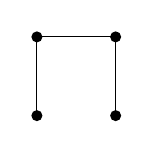
\begin{tikzpicture}

	\node (n1) at (0,0) {};
	\node (n2) at (1,0) {};
	\node (n3) at (1,1) {};
	\node (n4) at (0,1) {};

	\foreach \i in {1,...,4}
	{
		\fill (n\i) circle [radius=2pt];
	};

	\foreach \i / \j in {2/3, 3/4, 4/1}
	{
		\path (n\i.center) edge (n\j.center);
	};
	\end{tikzpicture}
	&
	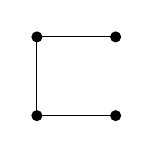
\begin{tikzpicture}

	\node (n1) at (0,0) {};
	\node (n2) at (1,0) {};
	\node (n3) at (1,1) {};
	\node (n4) at (0,1) {};

	\foreach \i in {1,...,4}
	{
		\fill (n\i) circle [radius=2pt];
	};

	\foreach \i / \j in {
	1/2, 
	%2/3, 
	3/4,
	4/1}
	{
		\path (n\i.center) edge (n\j.center);
	};
	\end{tikzpicture}
	&
	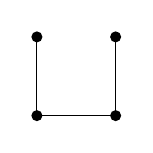
\begin{tikzpicture}

	\node (n1) at (0,0) {};
	\node (n2) at (1,0) {};
	\node (n3) at (1,1) {};
	\node (n4) at (0,1) {};

	\foreach \i in {1,...,4}
	{
		\fill (n\i) circle [radius=2pt];
	};

	\foreach \i / \j in {
	1/2, 
	2/3, 
	%3/4,
	4/1}
	{
		\path (n\i.center) edge (n\j.center);
	};
	\end{tikzpicture}
	&
	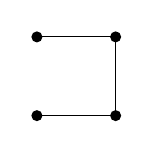
\begin{tikzpicture}

	\node (n1) at (0,0) {};
	\node (n2) at (1,0) {};
	\node (n3) at (1,1) {};
	\node (n4) at (0,1) {};

	\foreach \i in {1,...,4}
	{
		\fill (n\i) circle [radius=2pt];
	};

	\foreach \i / \j in {
	1/2, 
	2/3, 
	3/4}
	%4/1}
	{
		\path (n\i.center) edge (n\j.center);
	};
	\end{tikzpicture}
	\\
	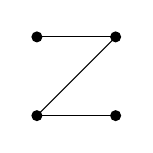
\begin{tikzpicture}

	\node (n1) at (0,0) {};
	\node (n2) at (1,0) {};
	\node (n3) at (1,1) {};
	\node (n4) at (0,1) {};

	\foreach \i in {1,...,4}
	{
		\fill (n\i) circle [radius=2pt];
	};
	\foreach \i / \j in {
	1/2, 
	%2/3, 
	3/4,
	%4/1,
	1/3}
	{
		\path (n\i.center) edge (n\j.center);
	};
	\end{tikzpicture}
	&
	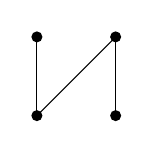
\begin{tikzpicture}

	\node (n1) at (0,0) {};
	\node (n2) at (1,0) {};
	\node (n3) at (1,1) {};
	\node (n4) at (0,1) {};

	\foreach \i in {1,...,4}
	{
		\fill (n\i) circle [radius=2pt];
	};
	\foreach \i / \j in {
	%1/2, 
	2/3, 
	%3/4,
	4/1,
	1/3}
	{
		\path (n\i.center) edge (n\j.center);
	};
	\end{tikzpicture}
	&
	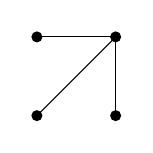
\begin{tikzpicture}

	\node (n1) at (0,0) {};
	\node (n2) at (1,0) {};
	\node (n3) at (1,1) {};
	\node (n4) at (0,1) {};

	\foreach \i in {1,...,4}
	{
		\fill (n\i) circle [radius=2pt];
	};
	\foreach \i / \j in {
	%1/2, 
	2/3, 
	3/4,
	%4/1,
	1/3}
	{
		\path (n\i.center) edge (n\j.center);
	};
	\end{tikzpicture}
	&
	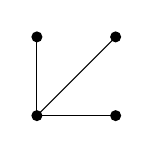
\begin{tikzpicture}

	\node (n1) at (0,0) {};
	\node (n2) at (1,0) {};
	\node (n3) at (1,1) {};
	\node (n4) at (0,1) {};

	\foreach \i in {1,...,4}
	{
		\fill (n\i) circle [radius=2pt];
	};
	\foreach \i / \j in {
	1/2, 
	%2/3, 
	%3/4,
	4/1,
	1/3}
	{
		\path (n\i.center) edge (n\j.center);
	};
	\end{tikzpicture}

	\end{tabular}
}
\caption{Graph $G$ and all its spanning trees}
\end{figure}





\begin{equation*}
\begin{array}{ll}
	\tilde A = \begin{pmatrix}
		0 & a & d & e \\
		a & 0 & 0 & b \\
		d & 0 & 0 & c \\
		e & b & c & 0 
	\end{pmatrix}
	&
	\tilde D = \begin{pmatrix}
		a+d+e \\
		& a+b \\
		& & c+d \\
		& & & b+c+e \\
	\end{pmatrix}
\end{array} 
\end{equation*}
\begin{equation*}
	\tilde D - \tilde A = \begin{pmatrix}
		\tikzmark{topA}a+\tikzmark{topA2}d+e & -a & -d & -\tikzmark{topB}e \\
		 -a & a+b & 0 & -b \\
		-d & 0 & c+d & -c \\
		-\tikzmark{botA}e & -b & -c & b+c+e \\
	\end{pmatrix}
\end{equation*}
\DrawLineHorizontal[red, thick, opacity=0.5]{topA}{topB}
\DrawLine[red, thick, opacity=0.5]{topA2}{botA}

\begin{equation*}
\begin{array}{ll}
\begin{vmatrix}
	a+b & 0 & -b \\
	0 & c+d & -c \\
	-b & -c & b+c+e
\end{vmatrix} 
& = (a+b)(c+d)(b+c+e)-b^2(c+d)-c^2(a+b) \\
& = bcd + abc+ abd +acd + ace + ade + bce + bde \\
& \text{every term represents a spanning tree}
\end{array}
\end{equation*}

if we set $a=b=c=d=1$ then

\begin{itemize}
	\item $\tilde A \rightarrow A$
	\item $\tilde D \rightarrow D = 
		\begin{pmatrix}3 \\ & 2 \\ & & 2 \\ & & & 3 \\ \end{pmatrix}$
	\item $\det{(D-A)'} = 8$
\end{itemize}

\textbf{Theorem (Kirchhoff's Matrix-Tree Theorem).}
Let
\begin{align*}
G &&& \text{undirected connected graph,} \\
A &&& \text{adjacency matrix,} \\
\operatorname{diag}(d(v_1),\ldots,d(v_n)) = D &&& \text{degree matrix,} \\
(D-A)' &&& \text{$D-A$ with one row and one column removed.}
\end{align*}
Then $|\det{(D-A)'}|$ is the number of spanning trees of $G$.

\textbf{Remark.} If $G$ is not connected, the number of spanning trees can be
found for each connected component. Multiply results to get the number
of possible combinations.


% Minimal or Maximal Spanning Tree
% sub problem
% Minimal or maximal Spanning Trees
\begin{figure}[htb]
\centering
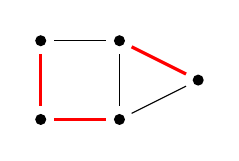
\begin{tikzpicture}[every node/.style = {circle}]

\node (a) at (0,0) {};
\node (b) at (1,0) {};
\node (c) at (2,0.5) {};
\node (d) at (1,1) {};
\node (e) at (0,1) {};
\foreach \node in {a,...,e}
{
	\fill (\node) circle [radius=2pt];
};

\draw[red,very thick] (a) -- (b);
\draw[red,very thick] (a) -- (e);
\draw[red,very thick] (c) -- (d);
%\draw (a) -- (b);
%\draw (a) -- (e);
\draw (b) -- (c);
\draw (b) -- (d);
%\draw (c) -- (d);
\draw (d) -- (e);
\end{tikzpicture}
\caption{Graph $G$ and its maximal spanning forest}
\end{figure}





% Proof: F_1, F_2 \sub E
% Observe:
% connecting the trees of a forest with edge e
\begin{figure}[htb]
\centering
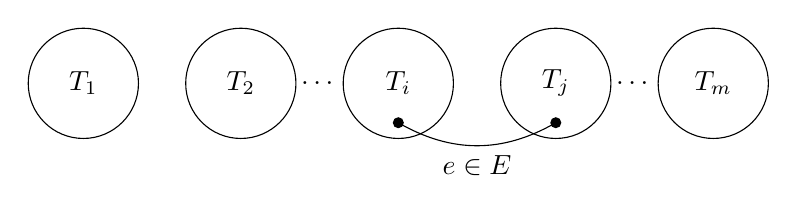
\begin{tikzpicture}
\node[] (T1) at (0,0) {$T_1$};
\node[] (T2) at (2,0) {$T_2$};
\node[] (T_dots1) at (3,0) {\ldots};
\node[] (Ti) at (4,0) {$T_i$};
\node[] (Tj) at (6,0) {$T_j$};
\node[] (T_dots2) at (7,0) {\ldots};
\node[] (Tm) at (8,0) {$T_m$};
\node[] (Ti_e) at (4,-0.5) {};
\node (Tj_e) at (6,-0.5) {};

\draw \foreach \n in {T1, T2, Ti,Tj,Tm}
{
	(\n) circle (0.7)
};

\fill (Ti_e) circle [radius=2pt];
\fill (Tj_e) circle [radius=2pt];

\path (Ti_e.center) edge [bend right] node[below] {$e \in E$} (Tj_e.center) ;

\end{tikzpicture}
\caption{Forest $F_2$ and its trees}
\end{figure}



\missingdate{2013-10-10}
\missingdate{2013-10-11}


\TODO{Missing parts from second week}
\section{Weighted Graphs and Algorithms}
\TODO{Missing parts from second week}
% Discrete Mathematics Lecture Notes 17.10.2013

% (Last week)

\subsection*{Maximal Flows}

\def\dminus{\ensuremath{d^{-}}}
\def\dplus{\ensuremath{d^{+}}}
\def\real{\mathbb{R}}
\def\natural{\mathbb{N}}
\def\Gammaplus{\ensuremath{\Gamma^{+}}}
\def\Gammaminus{\ensuremath{\Gamma^{-}}}

\begin{definition}
\index{flow network}
Let $G=(V,E,w)$ be a directed network with
\begin{compactitem}
\item a weight function $w: E\mapsto \real_0^{+}$,
\item a source $s: \dminus(s) = 0$ and
\item a sink $t: \dplus(t) = 0$.
\end{compactitem}
Then $(V, E, w, s, t)$ is a \dt{flow network}.
\end{definition}

\begin{definition}
\index{flow}
$\phi: E\mapsto \real$ is a \dt{flow} on $G$ if
\begin{align*}
  &\forall e\in E: 0 ≤ \phi(e) ≤ w(e)
     &&\text{feasability condition} \\
  &\forall x\in V\setminus\{s,t\}:
     \underbrace{\sum_{y\in \Gammaminus(x)} \phi(yx)}_{\text{in-flow}} =
     \underbrace{\sum_{y\in \Gammaplus(x)} \phi(xy)}_{\text{out-flow}}
     &&\text{flow conservation condition} \\
\end{align*}
\end{definition}

\begin{definition}
The \dt{size} or \dt{valuation} $v(\phi)$ of $\phi$ is
\[
  v(\phi) = \sum_{y\in \Gammaplus(s)} \phi(sy).
\]
\end{definition}

\TODO{Lemma+Proof out-flow of source = in-flow of sink}

% new content

\begin{definition}
\index{cut!of a flow network}
A partition $V=S \cup T$ ($S\cap T=\varnothing$) such that $s \in S, t \in T$
is called a \dt{cut} of $G$.
\end{definition}

\begin{definition}
\index{capacity!of a cut}
The \dt{capacity} $c(S,T)$ of a cut is given by
\[ c(S,T) = \sum_{x\in S, y\in T} w(xy). \]
\end{definition}

A cut $(S,T)$ is minimal if all cuts $(S',T')$ satisfy $c(S', T') \geq c(S,T)$.

\Lemma. Let $G$ flow network, $\phi$ flow on $G$, $(S,T)$ cut of G. Then
\[
v(\phi) = \underbrace{\sum_{x\in S, y\in T} \phi(xy)}_{\text{flow forward}}
        - \underbrace{\sum_{x\in T, y\in S} \phi(xy)}_{\text{flow backwards}}
\leq c(S,T).
\]
In particular,
\[
  \max_{\text{flow $\phi$}} v(\phi)\leq \min_{\text{cut $(S,T)$}} c(S,T).
\]

\Proof.
\[
    v(\phi) = \sum_{v\in S} \left(
        \sum_{x\in \Gamma^+(v)} \phi(vx)
      - \sum_{y\in \Gamma^-(v)} \phi(yv)
    \right)
\]
\TODO{add picture of edge}

For each vertex, we count flow on outgoing edges with positive and flow on
incoming edges with negative sign. We have the following cases:
\begin{itemize}
\item Flow with both endpoints in $S$; outgoing and ingoing cancel each other
\item Flow with starting point in $S$ and end point in $T$, counted positive
\item Flow with starting point in $S$ and end point in $S$, counted negative
\end{itemize}

Thus, we can rewrite $v(\phi)$:
\[
    v(\phi) = \sum_{x\in S, y\in T} \phi(xy)
            - \sum_{x\in T, y\in S} \phi(xy)
\]
Observe that in the first sum, all $\phi (xy) \leq w(xy)$. The second sum is
nonnegative: $0 \leq \phi (xy) \leq c(S,T)$.

Thus
\[
    v(\phi) \leq c(S,T).
\]

\begin{definition}
\index{augmenting path}
A path $P: s\rightarrow t$ (ignoring edge direction) is said to be an \dt{augmenting
path} with respect to a flow $\phi$ if $\phi(e) < w(e)$ on every forward edge
of $P$ and $\phi(e) > 0$ on every backward edge.
\end{definition}

\textbf{Theorem.}
Let $G$ flow network, $\phi$ flow on $G$. Then 
\[v(\phi)\text{ maximal} \iff \nexists\text{ augmenting path (w.r.t. $\phi$)}.\]

\ProofForward.
Suppose there is an augmenting path $P$. Then we choose
\begin{alignat*}{3}
    \delta' &= \min_{e \in P,\text{ forward}} w(e) - \phi(e) &\null> 0 \\
    \delta'' &= \min_{e\in P,\text{ backward}} \phi(e) &\null> 0 \\
    \delta &= \min(\delta', \delta'') &> 0
\end{alignat*}

Define
\[
    \tilde\phi := \begin{cases}
        \phi(e) + \delta &\text{if $e$ forward edge of $P$} \\
        \phi(e) - \delta &\text{if $e$ backward edge of $P$} \\
        \phi(e) &\text{otherwise}.
    \end{cases}
\]

$\tilde\phi$ is a flow on $G$.

Because we take the minimum of all the flows $\delta$, $\tilde\phi$ does not become negative on backward edges.

Because we increase the flow on the augmenting path by $\delta$,
\[
    v(\tilde\phi) = v(\phi) + \delta > v(\phi).
\]

\ProofBackward.
Assume there is no augmenting path. Let
\[
    S = \{v\in V \mid \exists\;\text{augmenting path $s\rightarrow v$}\}.
\]
There is no augmenting path $s\rightarrow t$, thus $t \notin S$.
Thus $(S, T = V\setminus S)$ is a cut.
Each edge $xy$ with $x\in S, y\in T$ must be saturated: otherwise it would be possible to find an augmenting path.

\TODO{add picture of S patch x edgy y in T}

Each edge $xy$ with $x\in T, y\in S$ must be void ($\phi(xy) = 0$). Thus
\[
    v(\phi) = c(S,T) - 0.
\]

Therefore $\phi$ must be maximal.

\textbf{Theorem.} If $G$ is a flow network such that $\forall e\in E': w(e)\in
\mathbb{N}$, a maximal flow exists.

\textbf{Proof.} $ \phi_{0}(e) \equiv 0$, if $\phi_{0}$ not max $\implies \exists$ augmenting path with $\delta \in \mathbb{N^{+}}$

Construct $\phi_1$ according to previous proof ($\tilde\phi$). We know that $v(\phi_1) ≥ 1$. Now we iterate and get $\phi_2, v(\phi_2) ≥ 2$,~\ldots After finitely many steps, we reach a flow $\phi_{\text{max}}$ where we cannot find an augmenting path anymore.

\textbf{Corollary.} If $G$ is a flow network with a weight function $w: E\mapsto \mathbb{Q}$, this implies $\exists\;\text{maximal flow}$.

\textbf{Remark.}
If weights are real, it can also be shown that a maximal flow exists (but you need a different proof strategy).

\textbf{Theorem (Max-flow/min-cut theorem).}
Let $G$ be a flow network $\implies \exists$ max. flow and $v(\phi_{\text{max}})= \min_{(S,T) cut} c(S,T)$

% slides: Algorithm of Ford-Fulkerson

\section{Special Graph Classes}

\subsection*{Eulerian Graphs}

\begin{definition}
A \dt{Eulerian trail}, which can be open or closed, is a trail where no edge is repeated and every edge is used. In a closed trail or \dt{Eulerian tour}, start = end.
\end{definition}

\begin{definition}
A graph is called \dt{Eulerian} if there is an Eulerian tour.
\end{definition}

\textbf{Theorem.}
Let $G=(V,E)$ be an undirected, connected multigraph. Then
\[
  G\text{ is Eulerian} \iff \forall x\in V: d(x)\text{ even}.
\]

There is an \emph{open} Eulerian trail $\iff$ exactly two vertices have odd degree.

\textbf{Proof.}
% "<==" direction
Proof by induction on $\alpha_1(G) =: m$.

$m = 0$: Trivial, only one vertex.

$m ≥ 1$: construct a tour $W$. You can always find a tour because degrees are even, thus every time you enter a vertice you can certainly find an edge where you can leave it.

Two cases:
a) $W$ is an Eulerian tour
b) $W$ is not an Eulerian tour

Then remove $W$, resulting in a graph $G'$ with connected components $G'_1$,~\ldots Then
\[
    \forall x\in V(G'_{i}): d_{G'}(x)\text{ is still even}
\]

Since all $G'_{i}$ are smaller than $G$, we can apply the induction hypothesis. This means $G'_{i}$ must be Eulerian (with Eulerian tours $W_{i}$.

$\forall i: W_i$ and $W$ have common vertex. Thus you can construct an Eulerian tour for the whole graph.

% Slides: Eulerian tour (started at 09:57... :)

% "==>" direction

Walk on an Eulerian tour. 













%\include{02_the_next_chapter}

\printindex

\end{document}
